\documentclass[openany,svgnames]{book}
\usepackage[svgnames]{xcolor}
\usepackage{blindtext}

\usepackage{comment}

\usepackage{parskip}
\setlength{\parindent}{0pt}

\usepackage{geometry}
\geometry{letterpaper, portrait, margin=0.5in}

\usepackage{imakeidx}
\makeindex[columns=3]

\usepackage{multicol}
\usepackage{enumitem}
\usepackage{tabularx}
\usepackage{nameref}
\usepackage{tikz}
\usepackage[sfdefault]{roboto}
\usepackage[most]{tcolorbox}
\tcbuselibrary{breakable}
\usepackage{booktabs}
\usepackage{xtab}
\usepackage{makecell}
\usepackage{wrapfig}

\usepackage{array,ragged2e}
\newcolumntype{L}{>{\RaggedRight\arraybackslash}X}

\usepackage{titlesec}

\usepackage{etoolbox}

\usepackage{xparse}

\def\defcolwidth{0.6cm}
\def\aq{\textbf{Adventure Quest }}

\setcounter{secnumdepth}{5}

%\DeclareRobustCommand{\indy}[2]{\index{\MakeLowercase{#1}}\textbf{#2}}
\DeclareDocumentCommand \indy { o m } {%
  \IfNoValueTF {#1} {%
    \lowercase{\def\temp{#2}}%
    %\expandafter\index\expandafter{\temp}
    \index{\temp}%
    \textbf{#2}\xspace%
    %\index{\MakeLowercase{#1}}\textbf{#1}%
  }{%
    \lowercase{\def\temp{#1}}%
    %\expandafter\index\expandafter{\temp}
    \index{\temp}%
    \textbf{#2}\xspace%
    %\index{\MakeLowercase{#1}}\textbf{#2}%
  }%
}
\DeclareDocumentCommand \indx { m } {%
    \lowercase{\def\temp{#1}}%
    \index{\temp}%
}


\DeclareRobustCommand{\STR}{\indy[strength!STR]{STR}}
\DeclareRobustCommand{\INT}{\indy[intelligence!INT]{INT}}
\DeclareRobustCommand{\PER}{\indy[perception!PER]{PER}}
\DeclareRobustCommand{\CSE}{\indy[common sense!CSE]{CSE}}
\DeclareRobustCommand{\HEA}{\indy[health!HEA]{HEA}}
\DeclareRobustCommand{\AGI}{\indy[agility!AGI]{AGI}}
\DeclareRobustCommand{\PWR}{\indy[power!PWR]{PWR}}
\DeclareRobustCommand{\COM}{\indy[comliness!COM]{COM}}
\DeclareRobustCommand{\WIL}{\indy[willpower!WIL]{WIL}}
\DeclareRobustCommand{\CDV}{\indy[combat defense!CDV]{CDV}}
\DeclareRobustCommand{\CM}{\indy[combat modifier!CM]{CM}}
\DeclareRobustCommand{\GDV}{\indy[grapple defense!GDV]{GDV}}
\DeclareRobustCommand{\GM}{\indy[grapple modifier!GM]{GM}}
\DeclareRobustCommand{\MDV}{\indy[missile defense!MDV]{MDV}}
\DeclareRobustCommand{\MM}{\indy[missile modifier!MM]{MM}}
\DeclareRobustCommand{\DP}{\indy[damage points!DP]{DP}}
\DeclareRobustCommand{\EP}{\indy[experience points!EP]{EP}}
\DeclareRobustCommand{\DU}{\indy[divine units!DU]{DU}}
\DeclareRobustCommand{\EU}{\indy[elemential units!EU]{EU}}
\DeclareRobustCommand{\LF}{\indy[life force!LF]{LF}}
\DeclareRobustCommand{\LOS}{\indy[line of sight!LOS]{LOS}}

\newcommand{\newacronymidx}[4][]{
    \newacronym{#2}{#3}{#4}
    \ifstrempty{#1}
        { \index{#3|see{\MakeLowercase{#4}}} }
        { \index{#3|see{#1}} }
}

\DeclareTotalTCBox{\tcdieroll}{ O{GreenYellow} v !O{} }{%
  leftrule=0mm,%
  rightrule=0mm,%
  toprule=0mm,%
  bottomrule=0mm,%
  rounded corners,%
  top=1pt,%
  bottom=0pt,%
  left=2pt,%
  right=2pt,%
  tcbox raise base,%
  boxsep=0mm,%
  nobeforeafter,%
  colback=white!40!#1,%
  colupper=black,%
  halign=center,%
  }{\textbf{\strut{#2}}}

\DeclareTotalTCBox{\tcdefine}{ O{DodgerBlue} v !O{} }{%
  leftrule=0mm,%
  rightrule=0mm,%
  toprule=0mm,%
  bottomrule=0mm,%
  rounded corners,%
  top=1pt,%
  bottom=0pt,%
  left=2pt,%
  right=2pt,%
  tcbox raise base,%
  boxsep=0mm,%
  nobeforeafter,%
  colback=white!30!#1,%
  colupper=black,%
  halign=center,%
  }{\textbf{\strut{#2}}}

\DeclareTotalTCBox{\tcpage}{ O{Crimson} m !O{} }{%
  leftrule=0mm,%
  rightrule=0mm,%
  toprule=0mm,%
  bottomrule=0mm,%
  rounded corners,%
  top=1pt,%
  bottom=0pt,%
  left=2pt,%
  right=2pt,%
  tcbox raise base,%
  boxsep=0mm,%
  nobeforeafter,%
  colback=white!50!#1,%
  colupper=black,%
  halign=center,%
  }{\textbf{\strut{Page #2}}}

\newtcolorbox{normbox}[1][]{%
  boxrule=0pt,%
  enhanced,
  title=\textbf{#1},%
  left=2pt,%
  right=2pt,%
  top=2pt,%
  bottom=1pt,%
  boxsep=2pt,%
  boxrule=0.6pt,%
  lefttitle=2mm,%
  righttitle=2mm,
  toptitle=1mm,%
  bottomtitle=1mm,%
  minipage boxed title,%
  hbox,%
  colbacktitle=Navy,%
  colback=white,%
  }

\newtcolorbox{normboxper}[2][]{%
  boxrule=0pt,%
  enhanced,
  title=\textbf{#2},%
  left=2pt,%
  right=2pt,%
  top=2pt,%
  bottom=1pt,%
  boxsep=2pt,%
  boxrule=0.6pt,%
  lefttitle=2mm,%
  righttitle=2mm,
  toptitle=1mm,%
  bottomtitle=1mm,%
  width=#1\linewidth,%
  %width=0.5\linewidth,%
  minipage boxed title,%
  %attach boxed title to top,%
  }


\begin{document}
\enlargethispage{1.5\baselineskip}
\raggedright
%\setlength{\multicolsep}{6.0pt plus 2.0pt minus 1.5pt}%
\titlespacing\section{0pt}{6pt}{6pt}
\titlespacing\subsection{0pt}{6pt }{6pt}
\titlespacing\subsubsection{0pt}{6pt}{6pt}
%\incantentry{Life Light}{Talisman/permament}{500}{20 / Rank}{2 Hours / Rank}{Target's blood\\
Silver dust
}{A small vial is filled with a mixture of silver dust and the blood of a targeted individual. The nomad holds the vial and touches the target during the creation of this talisman. The vial begins to glow softly with a silver glow, as long as the target is }
\begin{titlepage}
\begin{center}
\huge Adventure Quest\\
Jaern\\
\vspace*{1cm}
\normalsize a Role Playing System\\
\vspace*{1cm}
created by\\
Daniel Lawrence\\
\vspace*{1cm}
based on version published\\
April 5th, 2010\\
\vspace*{1cm}
modified by\\
Michael Lubert\\
\vspace*{1cm}
modified version publish date\\
\today
\end{center}
\end{titlepage}
First Edition

\vspace*{1cm}
\begin{tabular}{ l l }
First Printing: & July 1991\\
Second Printing: & September 1992\\
Third Printing: & November 1992\\
Fourth Printing: & September 1997\\
Fifth Printing: & August 1998\\
Sixth Printing: & July 1999\\
Seventh Printing: & March 2001\\
Eigth Printing: & August 2005
\end{tabular}

\vspace*{1cm}
Copyright 1989 – 2010 by Daniel M. Lawrence and Robert J. Blake\\
Copyright 2010-2024 by Greg Mowczko

\vspace*{0.5cm}
All Rights are reserved. No part of this publication may be reproduced, stored in a retrieval system, or transmitted, in any form, or by any means, electronic, photocopying, recording,
or otherwise, without prior written permission of the publisher.\\

\vspace*{1cm}
Published by Daniel M. Lawence and Robert J. Blake\\
Adventure Quest is a trademark owned by Daniel M. Lawrence\\

\vspace*{1cm}
Find\\
http://www.aquest.com/\\
on the Internet to recieve up to date information on all Adventure Quest games.
\include{dedication.tex}
\textbf{INTRODUCTION}

\textbf{Adventure Quest\textsuperscript{TM}} (\textbf{AQ} for short) is a role playing system in which you, through your game persona (adventurer), can experience all the thrills and perform deeds of derring-do in a fantasy world. It is like being the hero in an adventure novel, only, instead of just reading about what happens, your actions and decisions direct the storyline. You can destroy evil maidens, rescue fair dragons, or even be a knight in very dull armor. Your imagination is the only limit to what you can do while playing Adventure Quest.

As a player, you create an adventurer which you control. Another person, called the Game Master (GM), presents to you and other players a fantasy world of cities, towns, creatures, oppressive overlords, demanding temples, and lots of magic and treasure. You tackle adventures in this world to satisfy the personality and motives of your adventurer. Adventure Quest tm provides adventure in a variety of different settings (Games), each with its own history, customs, inhabitants, villains, and deities. 

This Game covers adventuring in JAERN, a distant fantasy world far in our future. Other Adventure Quest games include AQ/BRITANNIA, describing a world similar to the British Isles in t he mid 1200’s; AQ/KHEMET, providing adventure in a land akin to ancient Egypt; AQ/FREEZONE, a coorporate ruled gangland in the near future; and AQ/SPACE, for adventuring in the outer reaches of Interstellar Space among the Pan-Human Hegemony.

\textbf{Realism and Playability}

Adventure Quest/Jaern is a complete game; you do not have to buy any other books before beginning play. It contains all the necessary information for players to create and play their adventurers, and for Game Masters to design and maintain a campaign. Any game such as this must strike some kind of balance between realism and playability. The mechanics used in this manual lean heavily towards the latter, with the idea that you should spend your time roleplaying your creations, be you a player or Game Master, rather than wading through very complex rules for the sake of realism.

That said, we realize that some of you might be willing to make a different tradeoff. Where appropriate, optional rules are included offering different, but more complex, mechanics that arguably provide greater realism. The players and Game Master may choose which options to include to tailor the game to their liking. The cornerstone of \textbf{Adventure Quest\textsuperscript{TM}} games are flexibility. Much of the game book deals with the creation of personalities, creatures, magical items, etc. Examples are provided that you can use as is, but more importantly we tell you how to create your own that will automatically be balanced with the system.

\textbf{About Role Playing}

Playing Adventure Quest, like any role playing game, should be a fun and exciting experience. Your adventurer will likely encounter many unusual, exotic, and strange situations, people, and activities. Your adventurer may end up in conflict with, or allied to, an array of intelligent beings and creatures, many of which we might consider strange or even evil by today’s standard and mores. Please remember that this is "just a game." The authors in no way endorse or suggest that you act out any game-related actions or methods in the real world. Practice safe gaming, and leave the game and any enemies you make there behind you at the gaming table.

\textbf{How to Use this Book}
\begin{itemize}
\item All players and Game Masters should read Chapters 1 through 4 which deal with the creation and playing of adventurers.
\item Chapters 5 through 10 describe the world of Jaern, the setting for this game, and is therefore also pertinent for both players and Game Masters.
\item Chapters 11 through 27 present the magic available in AQ/Jaern. 
\begin{itemize}
\item Chapter 11 discusses nomadic mystiscism. 
\item Chapters 12 through 16 deal with elemental magic, and are therfore of primary interest to players whose adventurers use magician spells.
\item Chapters 17 through 27 deal with divine magic. Each deity has its own chapter, so these are of interest to any player whose adventurer follows a particular god or goddess.
\end{itemize}
\item Chapters 28 through 35 are meant primarily for the Game Master. They discuss creation of actors, creatures, and treasures, designing interesting and exciting adventures, adjudicating adventures, and how to maintain a campaign.
\end{itemize}

\textbf{Pronoun Gender}

Gender neutral pronouns are in use where applicable, updaing from the previous version's masculine pronoun usage.

\textbf{Updates Made in This Version}

The following are areas that I felt were either no longer in keeping with the world that I played, were wholely missing, or were conflicting within the text:
\begin{enumerate}
\item Slavery: In the original text, slavery is both depicted as a form of punishment (akin to an endentured labor) and as a chattel version of slavery in which slaves remain in servitude for life. Additionally, the original text includes statements both that children cannot be slaves and that they can be born into slavery. As slave labor was often relegated to the background of scenes when I played, I will be removing much of the supporting text for it and updating it to be more in line to be a limited time frame of endentured labor, with the punishment for crimes not being transferable to kin, save for the withholding of inheritance to cover debts. References to "slave" will be replaced with "prisoner."
\item Weapons: Many of the weapons seem to hold nonsensical values with regard to their (sparse) descriptions. I will be making efforts to update the weapon table to make sense.
\item Souls: Much of the writings of nomadic, divine, and elemental magic systems involve souls and those who have them. There are entire branches of necromancy devoted to it. However, there are odd gaps when it comes to elves. As a result, I have made a determination that spells and effects which remove or destroy a soul do not kill the target. Additionally, as there is some confusion on the difference between the mind/soul, specifically in regards to memory and personality, I have made the determination that those are part of the soul. This means that a being or creature who is able to move their soul to another body (which is without a soul) will possess all of their knowledge and skills, but is still bound by the physical characteristics of their new form (meaning they may be unable to wield a weapon they are proficient in or cast certain spells beyond their WIL).
\end{enumerate}

\textbf{Original Acknowledgements}

The list below is really just the beginning. Many people have contributed in different ways at different stages of this project. We would especially like to thank Mark Shoemaker for lots of zany ideas and style over many years, Bob Ferguson for his devotion in filling out thousands of forms, to Scott Delaney for fixing all our cars, to Tony Charlesworth for his endless time researching a world full of information, to Greg Mowzko for not letting a single error problem by no matter how insufferable it was, to Microsoft for their Access product that holds all of our databases, and to our good roleplaying friends in Lake Geneva, for providing us the motivation.

Robert J. Blake, my coauthor of this system, created most of the elemental spells, a lot of creatures, many skill descriptions and provided a sounding board for all the basic concepts behind our system. He provided endless encouragement to bring this project to pass. Robert ran the AD\&D Open Tournement at the Gencon Gaming convention for over a decade, overseeing uncountable details of scenario design and game master coordination. It was his experience which made it possible for us to create this system. Also our work on these concepts found its place in improving other systems in many ways. Sadly, we lost Robert at the beginning of the new millenium. He will be greatly missed.

\textbf{Design assistance:}\\
Daniel Lawrence\\
Robert J. Blake\\
Dana Hoggatt\\
Eric Delaney\\
Christopher Stanley\\
Steve Ames\\
Greg Mowczko\\

\begin{tabular}{ l l }
\textbf{Cover Art:} & Terry Pavlet\\
\textbf{Interior Art:} & Sean Cannon\\
 & Kirstein Jacobus\\
 & Scott Starkey\\
\textbf{Logo Design:} & Karen Klutzke\\
\textbf{Database Design:} & Daniel Lawrence\\
\end{tabular}

\textbf{Play Testers:}\\
\begin{tabular}{ l l l l }
Aaron K Alexander & Andrew Grey Smith & Andrew M Luers & Anthony C Brown\\
Anthony Charlesworth & Benjamin Wai & Bill Dorell & Brent D McLean\\
Brett Riester & Brian Cash & Calvin Krug & Charles Voelkel\\
Chris Esser & Daniel Lawrence & Terry Pavlet & Sean Cannon\\
Kirstein Jacobus & Scott Starkey & Karen Klutzke & Daniel Lawrence\\
Chris Normand & Craig Waylan & Dana Shea & David H Morse\\
David Moore & David Ward & Eric Starkey & Erich Shultz\\
Gregory Mowczko & Jeff Hartwig & Jim Ivey & Joe Gregorovich\\
Jose Berrios & John Flournoy & John Haley & John W. Fisher\\
John R. Prewitt III & Kat Price & Kathy Janney & Kirk Monsen\\
Lee Kenyon & Lyle H Janney & Mark Muller & Matthew W Somers\\
Michael Ballard & Michael Brobst & Patrick Collins & Patrick Perrone\\
Paul Bernard & Robert Tertocha & Robert Thelan & Robert Westerman\\
Ryan Gavigan & Ryan Parker & Scott Starkey & Sean L McLane\\
Steve Ames & Terran D Lane & Tessy E Fitzpatrick
\end{tabular}
\chapter{Creating an Adventurer}
\label{ch:create-adventurer}
To play in \textbf{Adventure Quest} (\textbf{AQ} for short), you must first create an adventurer to control during the game. All adventurers start out as young persons just leaving home, seeking fame, fortune and yet more adventure. Keep track of your adventurer’s attributes and skills by completing a 4x6 \textbf{adventurer card} like the empty one below; use a pencil for this, as frequent changes will be made during the adventurer’s career.

\begin{tabularx}{\textwidth}{ X l l l l }
\midrule\\
Name: & ( & ) & & Rate\\
STR & Background & & Mod / Defense & Date\\
INT & DP & Combat & / & Silver\\
PER & EU/DU & Missle & / & EXP\\
CSE & Element & Grapple & / & Profession\\
HEA & Languages: & Skills: & Equipment: & Enchanted Items:\\
AGI\\
PWR\\
COM\\
WIL\\[0.25cm]

Race\\
Sex\\
DoB\\
Age\\
Build\\
Height\\
Weight\\
Eye\\
Hair\\
Motive\\
Deity\\
\midrule
\end{tabularx}
\begin{multicols}{2}
\section{Random Numbers}
When people are born, they do not get to choose to be male or female, tall or short, or clever or daft. To simulate this in AQ, these attributes (and other uncontrollable random events) are determined by rolling dice. Later, you may freely choose the skills, languages, etc. your adventurer learns as he grows.\\
Dice come in many different sizes, and when a die roll is required, the type and number are expressed like this:\\
\begin{center}
(\# of dice) d (sides of dice)
\end{center}
Thus, "3d6" means to roll three six-sided dice and add up the results of each die to get the total result. Always assume six-sided dice if the number of sides per die is not specified.
\section{Physical Statistics}
Each adventurer has several attributes. The most important of these are the nine physical statistics or stats, which are listed at the top of the first column of the adventurer card. These stats normally have a rank or value between 0 and 24. These represent:

\begin{tabular}{p{0.2\linewidth} p{0.1\linewidth} p{0.6\linewidth}}
\textbf{Strength} & (STR) & Physical prowess\\
\textbf{Intelligence} & (INT) & Reasoning and problem solving\\
\textbf{Perception} & (PER) & Awareness of surrounding events\\
\textbf{Common Sense} & (CSE) & Sound practical judgement\\
\textbf{Health} & (HEA) & Physical well-being\\
\textbf{Agility} & (AGI) & Physical coordination\\
\textbf{Power} &  (PWR) &  Magical potential\\
\textbf{Comeliness} & (COM) & Physical beauty\\
\textbf{Willpower} & (WIL) & Mental strength\\
\end{tabular}

Each stat is generated by totalling the roll of 3d6, and thus ranges from 3 to 18. Roll 3d6 and write the total op posite STR on the card , roll aga in an d write the total opposite INT, etc. until all stats have a value. Do not despair if they are not all high; playing an adventurer with both strong and weak points is much more fun and interesting than playing an omnipotent adventurer who never needs to think.
\section{Placed Roll}
After rolling the stats, you may change them somewhat to fit the kind of adventurer you wish to play. Roll 4d6 and throw any one die out, totalling the remaining three. Use this total to replace the value of any of your nine original stats. If the roll is unsatisfactory, ignore it and leave your stats unchanged.
\section{Race}
Your adventurer may be one of five different races of intelligent creatures. Members of different races have differing physical appearances and abilities; see \textbf{Chapter \ref{ch:jaern-races}: \nameref{ch:jaern-races}} on page \textbf{\pageref{jh-races}}. Roll 1d20 and check on the following table to determine your adventurer’s race.
\begin{tcolorbox}[breakable,boxrule=0pt]
\begin{tabular}{l l}
Roll & Race\\
\midrule
01 - 14 & Human\\
15 & Elf\\
16 & Dwarf \\
17 & Lizard\\
18 & Orc\\
19 - 20 & Half-breed\\
\end{tabular}
\end{tcolorbox}
If the roll is 19 or 20 this means the adventurer’s parents were of different races. Now roll to find the race of each parent. Each must be a different race, of course, so if the second parent roll is the same as the first, roll again until a different race is determined. The parents may be half-breeds themselves, which means that the adventurer’s grandparents must be determined the same way. If a half-breed grandparent is rolled, ignore it and roll again. Racial heritage determines which racial skills your adventurer has. Non-physical differences are represented as racial skills. For each list below in which your adventurer has a grandparent, roll 1d4 for each skill. If the number is equal to or less than the number of grandparents of that race, write that skill on the adventurer card. If your adventurer is purebred, (i.e., all four grandparents are the same race) he automatically gets all that race's skills. Read the \textbf{Chapter \ref{ch:jaern-humanoids}: \nameref{ch:jaern-humanoids}} to learn about these skills and racial disadvantages.

\begin{multicols}{2}
\textbf{Elf}
\begin{enumerate}
\item Exceptional PER
\item Distance Judgment
\item Missile Skill*
\item Soulless
\end{enumerate}
\textbf{Orc}
\begin{enumerate}
\item Exceptional WIL
\item Enhanced Smell
\item Physical Viciousness*
\item Mental Stubbornness
\end{enumerate}
\textbf{Dwarf}
\begin{enumerate}
\item Exceptional HEA
\item Material Sense
\item Armor Construction*
\item Great Durability
\end{enumerate}
\textbf{Lizard}
\begin{enumerate}
\item Exceptional AGI
\item Quickness
\item Water Breathing
\item Homing
\end{enumerate}
\end{multicols}

*partial breeds check \textbf{Chapter \ref{ch:jaern-races}} to learn how to set these skills.
\nameref{ch:create-adventurer}

Elves are extremely long lived compared to the other races. The do not, however, posses a soul, and thus do not have an existance after death. This makes then unable to use divine magic, and unable to ever be brought back from the dead. Elves generally do not interact with the dieties and their priests. Holy places like temples and shrines make them feel uncomfortable and they tend to avoid them.\\
Full Humans are often more diverse and adaptable than other races. If your adventurer is a full bred human, you may take an additional Placed Roll to further customize your stats. Roll 4d6 and throw any one die out, to talling the remaining three. Use this total to again replace the value of any of your nine original stats. If the roll is unsatisfactory, ignore it and leave your stats unchanged.
\section{Sex}
Choose a sex for your adventurer, or roll 1d6 and
check against the following table:
\begin{tcolorbox}[breakable,boxrule=0pt]
\begin{tabular}{l l}
1 - 3 & Male\\
4 - 6 & Female
\end{tabular}
\end{tcolorbox}
\section{Age}
Determine how old your adventurer is at the start of his or her career by rolling one die of the appropriate type
(from the following table) for each grandparent, and add 10 to the result.
\begin{tcolorbox}[breakable,boxrule=0pt]
\begin{tabular}{l l}
\textbf{Race} & \textbf{Age Die}\\
\midrule
Orc & 4\\
Human & 6\\
Lizards &  8\\
Dwarf & 10\\
Elf &  20\\
\end{tabular}
\end{tcolorbox}
If your adventurer is pure human, obviously all four of his grandparents are human. Roll 4d6, total them and add 10 to find out his age. If, for example, he is half-elf, quarter-human and quarter-dwarf, roll 2d 20 + 1d6 + 1d10 + 10. Aging is covered in detail in \textbf{Chapter \ref{ch:jaern-humanoids}: \nameref{ch:jaern-humanoids}} on page \textbf{\pageref{jh-aging}}.
\section{Body build}
If your adventurer is not purebred, roll 1d4 to randomly select a grandparent’ s race. Now roll 1 d20 to determine your adventurer’s body build using the appropriate race column on the following table. If your adventurer is female, her body build is one catagory smaller than the chart result.
\begin{tcolorbox}[breakable,boxrule=0pt]
\begin{tabular}{l l l l l l}
 & Orc & Elf & Human & Dwarf & Lizard\\
\midrule
A & - & - & - & - & -\\
B & 1 & 1- 2 & - & - & -\\
C & 2- 5 & 3- 6 & 1- 2 & - & -\\
D & 6-16 & 7-14 & 3- 6 & 1 & 1- 2\\
E & 17-19 & 15-18 & 7-14 & 2- 5 & 3- 6\\
F & 20 & 19-20 & 15-18 & 6-16 & 7-14\\
G & - & - & 19-20 & 17-19 & 15-18\\
H & - & - & - & 20 & 19-20\\
\end{tabular}
\end{tcolorbox}
\end{multicols}
\section{Height and Weight}
Height and weight are determined by rolling 4d6 and totalling them. Add the number shown below for the race of each grandparent.
\begin{tcolorbox}[breakable,boxrule=0pt]
\begin{tabular}{l l}
Dwarves & +0\\
Orcs & +2\\
Humans & +4\\
Elves & +5\\
Lizards & +6\\
\end{tabular}
\end{tcolorbox}
\begin{center}
\large
Height and Weight Table\\
\end{center}
\normalsize
\begin{tcolorbox}[breakable,boxrule=0pt]
\begin{tabular}{l l l l l l l l l l}
ROLL & height & A & B & C & D & E & F & G & H\\
\midrule
4 & 3'7" & 29 & 35 & 42 & 51 & 62 & 74 & 89 & 108\\
5 & 3'8" & 31 & 37 & 44 & 54 & 65 & 78 & 94 & 113\\
6 & 3'9" & 32 & 39 & 47 & 56 & 68 & 81 & 98 & 118\\
7 & 3'10" & 34 & 40 & 49 & 59 & 71 & 85 & 103 & 124\\
8 & 3'11" & 35 & 42 & 51 & 61 & 74 & 89 & 107 & 129\\
9 & 4'0" & 37 & 44 & 53 & 64 & 77 & 93 & 112 & 135\\
10 & 4'1" & 38 & 46 & 55 & 67 & 80 & 97 & 117 & 141\\
11 & 4'2" & 40 & 48 & 58 & 70 & 84 & 101 & 122 & 146\\
12 & 4'3" & 41 & 50 & 60 & 72 & 87 & 105 & 127 & 153\\
13 & 4'4" & 43 & 52 & 63 & 75 & 91 & 109 & 132 & 159\\
14 & 4'5" & 45 & 54 & 65 & 78 & 94 & 114 & 137 & 165\\
15 & 4'6" & 47 & 56 & 68 & 81 & 98 & 118 & 142 & 171\\
16 & 4'7" & 48 & 58 & 70 & 85 & 102 & 123 & 148 & 178\\
17 & 4'8" & 50 & 60 & 73 & 88 & 106 & 127 & 153 & 185\\
18 & 4'9" & 52 & 63 & 75 & 91 & 110 & 132 & 159 & 192\\
19 & 4'10" & 54 & 65 & 78 & 94 & 114 & 137 & 165 & 199\\
20 & 4'11" & 56 & 67 & 81 & 98 & 118 & 142 & 171 & 206\\
21 & 5'0" & 58 & 70 & 84 & 101 & 122 & 147 & 177 & 213\\
22 & 5'1" & 60 & 72 & 87 & 105 & 126 & 152 & 183 & 220\\
23 & 5'2" & 62 & 75 & 90 & 108 & 130 & 157 & 189 & 228\\
24 & 5'3" & 64 & 77 & 93 & 112 & 135 & 162 & 196 & 236\\
25 & 5'4" & 66 & 80 & 96 & 116 & 139 & 168 & 202 & 243\\
26 & 5'5" & 68 & 82 & 99 & 119 & 144 & 173 & 209 & 251\\
27 & 5'6" & 70 & 85 & 102 & 123 & 148 & 179 & 215 & 259\\
28 & 5'7" & 73 & 88 & 105 & 127 & 153 & 184 & 222 & 268\\
29 & 5'8" & 75 & 90 & 109 & 131 & 158 & 190 & 229 & 276\\
30 & 5'9" & 77 & 93 & 112 & 135 & 163 & 196 & 236 & 285\\
31 & 5'10" & 80 & 96 & 115 & 139 & 168 & 202 & 243 & 293\\
32 & 5'11" & 82 & 99 & 119 & 143 & 173 & 208 & 251 & 302\\
33 & 6'0" & 84 & 102 & 122 & 148 & 178 & 214 & 258 & 311\\
34 & 6'1" & 87 & 105 & 126 & 152 & 183 & 220 & 266 & 320\\
35 & 6'2" & 89 & 108 & 130 & 156 & 188 & 227 & 273 & 329\\
36 & 6'3" & 92 & 111 & 133 & 161 & 194 & 233 & 281 & 339\\
37 & 6'4" & 94 & 114 & 137 & 165 & 199 & 240 & 289 & 348\\
38 & 6'5" & 97 & 117 & 141 & 170 & 205 & 246 & 297 & 358\\
39 & 6'6" & 100 & 120 & 145 & 174 & 210 & 253 & 305 & 368\\
40 & 6'7" & 102 & 123 & 149 & 179 & 216 & 260 & 313 & 377\\
41 & 6'8" & 105 & 127 & 153 & 184 & 222 & 267 & 322 & 388\\
42 & 6'9" & 108 & 130 & 157 & 189 & 227 & 274 & 330 & 398\\
43 & 6'10" & 111 & 133 & 161 & 194 & 233 & 281 & 339 & 408\\
44 & 6'11" & 114 & 137 & 165 & 199 & 239 & 288 & 348 & 419\\
45 & 7'0" & 117 & 140 & 169 & 204 & 246 & 296 & 356 & 429\\
46 & 7'1" & 119 & 144 & 173 & 209 & 252 & 303 & 365 & 440\\
47 & 7'2" & 122 & 148 & 178 & 214 & 258 & 311 & 374 & 451\\
48 & 7'3" & 125 & 151 & 182 & 219 & 264 & 318 & 384 & 462\\
\end{tabular}
\end{tcolorbox}
\pagebreak
\begin{multicols}{2}
\normalsize
\section{Eye color}
If your adventurer is not purebred, roll 1d4 to randomly select a grandparent's race. Now roll 1d20 to find your adventurer's eye color, using the apropriate race column on this table:

\begin{tcolorbox}[breakable,boxrule=0pt]
\begin{tabular}{l l l l l l}
Color & Human & Elf & Dwarf & Orc & Lizard\\
\midrule
Black & 1 & 1-2 & 1-10 & 1-4 & 1-12\\
Brown & 2-8 & -- & 11-18 & 5-6 & --\\
Blue & 9-14 & 3-10 & -- & -- & 13-15\\
Green & 15-16 & 11-14 & 19-20 & 7-12 & 16\\
Red & -- & 15-17 & -- & 13-18 & 17-19\\
Silver & -- & 18-19 & -- & -- & 20\\
Hazel & 17-20 & -- & -- & 19-20 & --\\
White & -- & 20 & -- & -- & --
\end{tabular}
\end{tcolorbox}

\section{Hair color}
If your adventurer is not purebred, roll 1d4 to randomly select a grandparent's race. Now roll 1d20 to find your adventurer's hair color, using the apropriate race column on this table:
\begin{tcolorbox}[breakable,boxrule=0pt]
\begin{tabular}{l l l l l l}
Color & Human & Elf & Dwarf & Orc & Lizard\\
\midrule

Brown & 1-7 & -- & 1-10 & 1-2 & --\\
Black & 8-11 & 1-6 & 11-16 & 3-16 & --\\
Blond & 12-15 & 7-8 & -- & -- & --\\
Red & 16-17 & 9-13 & 17 & 17-18 & --\\
Green & -- & 14-15 & -- & 19 & --\\
Grey & 18 & -- & 18 & -- & --\\
White & 19 & 16-18 & -- & 20 & --\\
None & 20 & -- & 19-20 & -- & 1-20\\
Silver & -- & 19-20 & -- & -- & --
\end{tabular}
\end{tcolorbox}
\section{Motivation}
That takes care of the random elements of adventurer creation; now you have a free hand in developing your adventurer’s inner-self. Evolving his personality takes some thought, but it is a rewarding aspect of roleplaying. A good way to start is to create an event that occurred early in his life that now defines his basic motivation. Once you have a starting point it is easier to describe more about their personality.
Below are some possible motivations from which to choose, but you are free to make up others as best fits your needs and concepts. Now mentally describe an event or condition to explain why it is your adventurer's primary motivation. Write this motive down on the Adventurer Card after "Motive." Here are some suggestions:

\begin{tabular}{l l}
Duty & Alliegance to a higher authority\\
Fame & Gaining recognition from others\\
Justice & Maintaining balance\\
Knowledge & Learning for learning’s sake\\
Passion & Serving a cause with intense emotional fervor\\
Pleasure & Seeking pleasures of the flesh\\
Power & Forcing the submission of others\\
Religion & Devoting their life to a higher authority\\
Righteousness & Striving to helpmankind\\
Romance & Earning the love and/or respect of others
\end{tabular}

The motive you choose is not meant to be a "straight jacket" to force you to play the adventurer within narrow bounds. It is meant to be used, by you, to help set a direction for your adventurer’s actions and a start for his personality. You always have the freedom to write down what you believe is your adventurer’s driving force on your card. Also realize that there is magic which can be used to determine your motive, and the results of this magic will be what is percieved by the GM as your motive, which may disagree with what you have written.
To learn more about creating your adventurer's personality, read \textbf{Chapter \ref{ch:creating-actors}: \nameref{ch:creating-actors}} to see how the GM creates personalities for actors. These methods are applicable to your adventurer’s personality as well.
\section{Patron Gods}
You may select one deity as your adventurer’s patron god. Adventurers aligning themselves to a deity this way are expected to assist the causes of the god, and especially to follow that god’s precepts and laws. In return, they are often assisted by the priests and followers of that deity. Worshipping more than one god is possible, but can become difficult if the deities conflict in any way. Write down the name(s) of the deity(s) on the adventurer card after "Deity." Here is a list of available deities; each is covered in detail in its own chapter.

\begin{tabular}{l l l}
\textbf{GOD} & \textbf{Sphere of Influence} & \textbf{Sex}\\
Ra & Bearer of Light & M\\
Isis & Mistress of Life & F\\
T’or & The Thunder of Righteousness & M\\
At’ena & Mistress of Wisdom & F\\
Osiris & Protector of Nature & F\\
Tarus & Master Archivist & M\\
Neptune & Dweller of the Waters & M\\
Orus & The Flame of Zeal & M\\
Anubis & Lord of the Dead & M\\
Rudri & Dweller of the Dark & F\\
Scrogg & Concubine and follower of Orus & M\\
\end{tabular}
\section{Adventurer Background}
Backrounds are the adventuring professions available in a specific AQ Game. Each Game has at least three major, divergent disciplines that may be followed, and thus gives three professions. Others are derived by combining two of the major disciplines to yield another, unique background.\\
It may be helpful for you to visualize this as a three-spoked wheel, each spok labeled witha a major discipline. In AQ/Jaern these are Combat, Magic, and Skills.

\begin{center}

\tikzset{every picture/.style={line width=0.75pt}} %set default line width to 0.75pt        

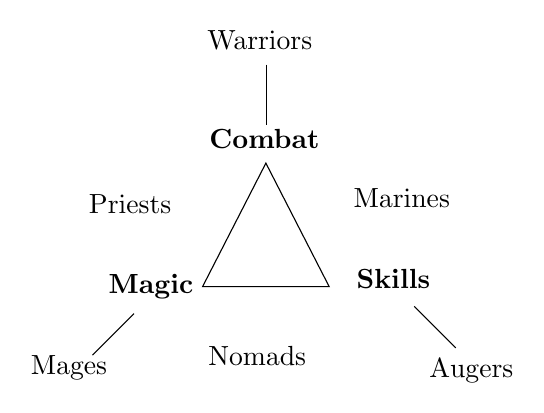
\begin{tikzpicture}[x=0.75pt,y=0.75pt,yscale=-1,xscale=1]
%uncomment if require: \path (0,300); %set diagram left start at 0, and has height of 300

%Straight Lines [id:da5792073549069615] 
\draw    (321.5,53) -- (321.5,82) ;
%Shape: Triangle [id:dp9921269194788708] 
\draw   (321,100.5) -- (351.5,160) -- (290.5,160) -- cycle ;
%Straight Lines [id:da10414083526965556] 
\draw    (257.5,173) -- (237.5,193) ;
%Straight Lines [id:da8045071749370871] 
\draw    (392.5,169.5) -- (412.5,189.5) ;

% Text Node
\draw (291.5,35.5) node [anchor=north west][inner sep=0.75pt]   [align=left] {Warriors};
% Text Node
\draw (234.5,114.5) node [anchor=north west][inner sep=0.75pt]   [align=left] {Priests};
% Text Node
\draw (362,111.5) node [anchor=north west][inner sep=0.75pt]   [align=left] {Marines};
% Text Node
\draw (206.5,192) node [anchor=north west][inner sep=0.75pt]   [align=left] {Mages};
% Text Node
\draw (292,187.5) node [anchor=north west][inner sep=0.75pt]   [align=left] {Nomads};
% Text Node
\draw (398.5,193.5) node [anchor=north west][inner sep=0.75pt]   [align=left] {Augers};
% Text Node
\draw (363.5,150.5) node [anchor=north west][inner sep=0.75pt]   [align=left] {\textbf{Skills}};
% Text Node
\draw (244,153) node [anchor=north west][inner sep=0.75pt]   [align=left] {\textbf{Magic}};
% Text Node
\draw (292.5,83) node [anchor=north west][inner sep=0.75pt]   [align=left] {\textbf{Combat}};


\end{tikzpicture}
\end{center}

The three backgrounds at the ends of the spokes are thus Warrior (for those exclusively trained in combat) Mages (Magic), and Augers (Skills). As for the areas between the spokes, a background that combines Magic and Combat produces the Priest, someone with a knowledge of Magic and the physical training to back it up. Combining Magic and skills yields a Nomad, with training in the mystical arts as well as skills. And finally, mixing Combat and Skills produces a Marine, a person with a need for fighting ability and quick and nimble movements.

\begin{tabular}{l l}
\textbf{Adventurer Background} & \textbf{Most Important Stat}\\
\midrule
Warrior & CSE and STR\\
Priest &  PWR and CSE\\
Magician &  PWR and INT\\
Nomad &  PER and HEA\\
Auger &  INT and CSE\\
Marine &  AGI and STR
\end{tabular}

Each background has one or more stats that is very important to the successful practice of the profession, as given in the above table. If your adventurer’s highest stat is
STR, they probably would fare best as a Warrior. If they have a high PER, you probably should consider making them a Nomad, etc.\\
You must now choose an available background for your adventurer. Consider not only the stats, but also what you envision your persona becoming, or what you want to roleplay. You are not forced to pick the background that matches the highest stat. In fact, successfully roleplaying (for example) an adventurer with a high STR and a mediocre INT as a Auger rather than a Warrior is very rewarding, not to mention entertaining, to you, the GM, and other players.Here are descriptions of the available backgrounds to further help you make a selection:\\
\begin{itemize}
\item A \textbf{Warrior} relies upon their skill at arms. They are proficient at fighting and confident in their ability to succeed with force. While they might serve in an army, a warrior prefers individual combat and is more likely found employed as a bodyguard, mercenary, constable, or a guard.
\item A \textbf{Priest} is devoted to the service of a deity, forever at that deity's disposal to spread their faith and worship throughout the world. A priest is willing for fight for their deity’s cause, but can also use god-given magical powers to further their goals.
\item A \textbf{Magician} is a practitioner of one of four types of elemental magics, using his magics to affect the world and gain wealth, recognition and influence. A magician is often consulted and employed by others to accomplish their goals.
\item The spells available in each element give a definite flavor to the personality and style of play of a magician. Fire and Air magicians tend to have more offensive spells, whereas Earth and Water mages are more defense oriented. Fire and Earth magic tends to be more individual in nature, while many Air and Water spells are useful to support and maintain a group of adventurers. If your adventurer is going to become a magician, bear these generalities in mind to select the elemental style that matches your adventurer's personality.
\item Brought up learning to think to solve their problems, an Auger’s basic tenet is to live up to their potential, learning to utilize their best skills and making the most of any situation.
\item Born to the seas, a \textbf{Marine} is a member of the traveling armies that plies the seas of Jaern. Ready with a quick story of marine heroes of the past, today's marine attempts to make a name for themseves and their shipmates. They adventure for fame, and are always ready for a good fight and a large tankard of ale.
\item Members of a tight-knit group of families, \textbf{Nomads} mistrust all other Jaernians and rarely travel among them. They are rumored to have various mystical and magical powers, so most people shun them, unsure of their intentions.
\end{itemize}
After choosing one of these, place it on the adventurer card after "Background." If you’re still uncertain, scan the list of Model Adventurers beginning on page \textbf{\pageref{adventurer-models}} for ideas and suggestions.\\
If it appears your adventurer suffers from hopelessly inadequate stats, they would probably not become an adventurer in a fantasy world. Ask the GM; they may allow you to discard this would-be adventurer and start over.
\section{Languages}
You need to know which languages (if any) your adventurer speaks to know how they can communicate with actors and other adventurers. Knowledge of languages is an intelligence-based skill, and beginning adventurers may know zero, one or two languages.
\begin{tcolorbox}[breakable,boxrule=0pt]
\begin{tabular}{l l l}
INT & Initial Languages & Maximum Languages\\
\midrule
3 - 5 & 0 & 0\\
6 - 8 & 1 & 1\\
9 - 11 & 2 & 2\\
12 - 14 & 2 & 3\\
15 - 17 & 2 & 4\\
18 - 20 & 2 & 5\\
21 - 23 & 2 & 6\\
24+ & 2 & 7\\
\end{tabular}
\end{tcolorbox}
Adventurers having an INT of less than 6 cannot speak coherently. They may know how to say isolated wordsor phrases, and can generally understand simple sentences. Playing adventurers with a low INT is very challenging because the player must communicate through actions rather than words. \\
The first language an adventurer with an INT greater than 6 learns is his racial language. This is Paroli for all human adventurers. Half-breed adventurers may pick one of their racial languages as their native tongue or the tongue of whomever raised him, whichever is most appropriate. The first language is always known at a skill rank of 9 or the adventurer’s INT, whichever is lower.\\
With an INT above 8, the player may choose a second language. For non-human adventurers, it would be prudent to pick the common tongue of the area to simplify communications. This second language is initially known at a skill rank of 6.

The available languages are:

\begin{tabular}{p{0.2\linewidth} p{0.7\linewidth}}
Breziak & human tongue\\
Dwarvish & race tongue of dwarves\\
Elvish & race tongue of most elves\\
Entish & spoken by intelligent forest creatures\\
Ferric & human tongue\\
Geleik & tongue of the elves of Silvan Isle\\
Haoogh & speech of the southern pirates\\
Orcish & race tongue of orcs\\
Paroli & race tongue for humans and common tongue\\
Sel’ict & race tongue of the lizard men\\
Trejon & ancient human tongue\\
\end{tabular}
\section{Rating}
Your GM must be able to balance your adventuring party against some opponents it might meet. Your adventurer's \textbf{Rating} is how many adventurers they have experienced. Set this at two now, and each time he finishes a gaming session, add one. A starting rating of two represents the skills that you choose in creating your adventurer. Your GM may ask for this number from all the players at the beginning of a gaming session.
\section{Date}
At the beginning and end of each adventure, the Game Master will tell you the current game date. The amount of time elapsed between adventures is important for curing damage, doing research, being pregnant, etc. The date is in ISO 8601 format (Year-Month-Day), such as 10080-06-15 SF (Since Founding). Record the current date minus your age on your card as your date of birth (DOB).
\section{Nomadic Prefix Names}
If your adventurer is a nomad, then they must know their own prefix name, or \textbf{epokonom}. Roll 1d20 and look at this table:
\begin{tcolorbox}[breakable,boxrule=0pt]
\begin{tabular}{l l|l l}
Roll & Epokonom & Roll & Epokonom\\
\midrule
1 - 5 & Raz- & 16 & Ald-\\
6 - 9 & Car- & 17 & Edo-\\
10 - 12 & Oka- & 18 & Ijo-\\
13 - 14 & Vem- & 19 & Bez-\\
15 & Lar- & 20 & Sag-\\
\end{tabular}
\end{tcolorbox}
Put this prefix before your adventurer’s name.
\section{Name}
Each adventurer must have a name of some sort. Choose a name for your adventurer and place it in the upper left-hand corner of the card. After this put your real name in parenthesis. This will help the Game Master to remember whose adventurer is whose.
\section{Profession}
Your adventurer may have a regular job to bring in a steady income. After your adventurer’s skills are selected (see page \textbf{\pageref{create-skills}}), you may choose one as their profession.
\section{Adventurer Models}
Players buy attributes for their adventurers using experience points. Physical equipment is bought with silver pieces. This buying allows you to make your adventurer’s abilities fit your perception of her personality.\\
To simplify making a new adventurer, several different Model Adventurers are reproduced here. If you wish to pick one of these, just copy the information from the chosen model that matches your adventurer’s background onto an adventurer card. For each defense value listed in the model, plug in the appropriate stats from your adventurer (dividing them by 5 and rounding down as shown) and add the results to find the your adventurer’s defense values. If they are an elf, add one on their MDV for Exceptional PER. If they are an orc, add one to his GDV for Exceptional WIL. Your adventurer is ready to play.\\
Each model allows you 20\% more attributes than if you had bought all the attributes separately. This extra does not make the adventurer more powerful; it is used to buy attributes that give added flavor and a direction for further development. Once selected, models cannot be modified or changed except to buy new attributes (or upgrade current ones) with earned experience points (see \nameref{create-buying} on page \textbf{\pageref{create-buying}}).
If none of the models fit your idea of your adventurer’s personality, and your GM is allowing custom a dventurer creation, skip this section and read \nameref{create-buying} to learn how to complete your adventurer’s creation.\\
Each adventurer prototype specifies the values for the following attributes:
\end{multicols}
\begin{tabular}{l l}
Damage Points (DP) & Relative health\\
Combat Modifier (CM) & Ability using hand-to-hand weapons\\
Missile Modifier (MM) & Ability using bows, slings and crossbows\\
Grapple Modifier (GM) & Ability to grapple\\
Spell type & Declared type of spells (EARTH, FIRE, AIR, WATER, and DIVINE)\\
Spell Groups & Ability to use various spell groups\\
Incants & Specific nomadic items and tailsmen\\
Skills & Purchased skills and their ranks\\
Combat Defense (CDV) & Resistance to being struck\\
Missile Defense (MDV) & Resistance to being hit by missiles\\
Grapple Defense (GDV) & Resistance to being grappled\\
\end{tabular}
\begin{multicols}{2}
\subsection{Models}
TBD
\section{Experience Points}
Experience Points (EP) are the currency used to buy such attributes as skills, stats, spells groups, damage points, and melee modifiers. Your adventurer is awarded EP during and after an adventure in several ways, depending on the method chosen by your GM. Using experience points in this way simulates any training or study that might be required to acquire or improve an ability without actually going through the tedium and boredom of doing so during a gaming session. By the way, when an adventure ends, don’t forget to add one to the Rating entry on the adventurer’s card. Your GM uses the Rating to get a rough idea of how much experience your adventurer has had so that they may balance the difficulty of an adventure against the power of the adventurers.\\
You may specify that a portion of the awarded experience be set aside and used later to buy attributes. There is no limit to the amount of experience your adventurer may hold, but it makes little sense to hold it longer than needed to buy the attributes sought.
\section{Buying}
\label{create-buying}
If you have not chosen an Adventurer Model, your adventurer is given 5,000 EP with which to buy:

\begin{tabular}{l l}
STATS & such as STR, INT, etc.\\
DAMAGE POINTS  & the ability to survive injury\\
MELEE MODs & abiltiy to resist physical damage\\
SPELLS & magician and priest magic\\
INCANTS & nomadic rituals\\
LANGUAGES & spoken languages\\
ABILITIES & useful skills and abilities\\
\end{tabular}

All buying must be done either when creating an adventurer or between adventures, and must be witnessed by the GM or their representative. The majority of the time this will be done when the adventurer has returned to a civilized setting, where the resources for training are most likely to be found. If an adventure is one in a series, and no game time has passed since the previous adventure, your GM may disallow buying attributes until after the entire sequence of adventures has been completed. \\
All attributes start at an initial rank of zero and may be bought upward one point at a time. To buy new attributes, or increase the value of an old one, multiply the base cost of the attribute by the point value you wish your adventurer to gain.

\textit{If Marna (a priestess of Osiris) attempts to raise her teaching skill (base cost 100 EP) from 8 to 9, she must expend 100 x 9 or 900 EP to do so.\\
If George the Magnificient (a Warrior) wants to raise his disguise attribute (base cost 50 EP) from 11 to 12, it will cost him 12 x 50 x 3 or 1800 EP. The 3x multiplier is included because the skill is an Auger skill, and George is a Warrior. See \nameref{create-skills} on page \textbf{\pageref{create-skills}} for more information on purchasing skills outside your class.}
\subsection{Buying up from zero}
While attributes are usually bought one point at a time, sometimes it is necessary to buy one from zero up to a high value. To do this, we use a little bit of math . . .\\
To buy something from zero to an arbitrary value, call that value N,

$Total Cost = \frac{N * (N+1)}{2} * Base Cost$

For example, to buy damage points (base cost 25 EP) from zero up to 16 would cost as follows:

$\frac{16 * (16+1)}{2} * 25 = \frac{16*17}{2} * 25 = 3,400 EP$

If the formula above is too intimidating, use the following table. Cross reference your adventurer’s current rank in the attribute against the desired rank, then multiply the number from the table by the base cost of the attribute to find the experience point cost.

\end{multicols}
\begin{tcolorbox}[breakable,boxrule=0pt]
\begin{tabular}{l l l l l l l l l l l l l l l l l l l}
\textbf{OLD} & \multicolumn{16}{c}{\textbf{NEW RANK}}\\
\textbf{RANK} & \textbf{1} & \textbf{2} & \textbf{3} & \textbf{4} & \textbf{5} & \textbf{6} & \textbf{7} & \textbf{8} & \textbf{9} & \textbf{10} & \textbf{11} & \textbf{12} & \textbf{13} & \textbf{14} & \textbf{15} & \textbf{16} & \textbf{17} & \textbf{18}\\
0 & 1 & 3 & 6 & 10 & 15 & 21 & 28 & 36 & 45 & 55 & 66 & 78 & 91 & 105 & 120 & 136 & 153 & 171\\
1 & -- & 2 & 5 & 9 & 14 & 20 & 27 & 35 & 44 & 54 & 65 & 77 & 90 & 104 & 119 & 135 & 152 & 170\\
2 & -- & -- & 3 & 7 & 12 & 18 & 25 & 33 & 42 & 52 & 63 & 75 & 88 & 102 & 117 & 133 & 150 & 168\\
3 & -- & -- & -- & 4 & 9 & 15 & 22 & 30 & 39 & 49 & 60 & 72 & 85 & 99 & 114 & 130 & 147 & 165\\
4 & -- & -- & -- & -- & 5 & 11 & 18 & 26 & 35 & 45 & 56 & 68 & 81 & 95 & 110 & 126 & 143 & 161\\
5 & -- & -- & -- & -- & -- & 6 & 13 & 21 & 30 & 40 & 51 & 63 & 76 & 90 & 105 & 121 & 138 & 156\\
6 & -- & -- & -- & -- & -- & -- & 7 & 15 & 24 & 34 & 45 & 57 & 70 & 84 & 99 & 115 & 132 & 150\\
7 & -- & -- & -- & -- & -- & -- & -- & 8 & 17 & 27 & 38 & 50 & 63 & 77 & 92 & 108 & 125 & 143\\
8 & -- & -- & -- & -- & -- & -- & -- & -- & 9 & 19 & 30 & 42 & 55 & 69 & 84 & 100 & 117 & 135\\
9 & -- & -- & -- & -- & -- & -- & -- & -- & -- & 10 & 21 & 33 & 46 & 60 & 75 & 91 & 108 & 126\\
10 & -- & -- & -- & -- & -- & -- & -- & -- & -- & -- & 11 & 23 & 36 & 50 & 65 & 81 & 98 & 116\\
11 & -- & -- & -- & -- & -- & -- & -- & -- & -- & -- & -- & 12 & 25 & 39 & 54 & 70 & 87 & 105\\
12 & -- & -- & -- & -- & -- & -- & -- & -- & -- & -- & -- & -- & 13 & 27 & 42 & 58 & 75 & 93\\
13 & -- & -- & -- & -- & -- & -- & -- & -- & -- & -- & -- & -- & -- & 14 & 29 & 45 & 62 & 80\\
14 & -- & -- & -- & -- & -- & -- & -- & -- & -- & -- & -- & -- & -- & -- & 15 & 31 & 48 & 66\\
15 & -- & -- & -- & -- & -- & -- & -- & -- & -- & -- & -- & -- & -- & -- & -- & 16 & 33 & 51\\
16 & -- & -- & -- & -- & -- & -- & -- & -- & -- & -- & -- & -- & -- & -- & -- & -- & 17 & 35\\
\end{tabular}
\end{tcolorbox}
\begin{multicols}{2}
\section{Stats}
Of all the attributes, stats are arguably the most important. Stats are the basis for most resistance checks (the avoidance of effects), and determine the maximum value for most other attributes (skills, languages, spell groups, etc.). At a base cost of 500, they are also very expensive to increase. For example, to buy STR from 14 to 15 would cost 500 x 15 = 7,500 experience points.
\hrule
\textit{Optional:\\
A physical stat may not be increased more than 4 above the initial roll, to reflect the notion that training and practice can only increase a physical ability so much.}
\hrule
\section{Damage Points}
Damage points (DP) indicate your adventurer's ability to avoid damage during combat. As you buy this total higher, your adventurer becomes more skillful at dodging, moving and twisting to avoid being damaged while fighting. If they are injured, damage points are temporarily subtracted from their totral DP; the new total indicates their relative condition.
Lost DP may be regained by resting. A full night’s rest (at least eight hours; twelve for those with no soul, like elves) restores a number of DP equal to the adventurer’s HEA divided by five (by two for those with the Exceptional HEA skill, like most dwarves), rounded down. Damage points may not be restored beyond the original maximum DP total. \\
The base cost for DPs is 25. Your adventurer must have DPs to survive, so here is a chart of the total cost of buying damage points up from zero.

\begin{tcolorbox}[breakable,boxrule=0pt]
\begin{tabular}{l l|l l|l l}
DP & Cost & DP & Cost & DP & Cost\\
\midrule
1 & 25 & 8 & 900 & 15 & 3000\\
2 & 75 & 9 & 1125 & 16 & 3400\\
3 & 150 & 10 & 1375 & 17 & 3825\\
4 & 250 & 11 & 1650 & 18 & 4275\\
5 & 375 & 12 & 1950 & 19 & 4750\\
6 & 525 & 13 & 2275 & 20 & 5250\\
7 & 700 & 14 & 2625 & 21 & 5775\\
\end{tabular}
\end{tcolorbox}

Buying damage points with experience actually simulates additional training to avoid being wounded. This could be handled as another defensive modification, but being able to take more damage yields the same effect, is easier to keep track of, balances quite nicely, and is more fun to play.\\
When buying damage points, you are only increasing your adventurer’s maximum DP, not their current DP total. New DPs are only gained after resting, according to the DP recovery rule above.
\section{Melee Modifiers}
Every adventurer has three modifiers, or Mods, that help determine success in combat. The \textbf{Combat Modifier (CM)} is added to all 1d20 "to strike" rolls you make when
your adventurer attacks using a hand-to-hand weapon. The \textbf{Missile Modifier (MM)} is added to all "to hit" rolls from bows, crossbows and thrown objects. The \textbf{Grapple Modifier (GM)} is used when wrestling or boxing an opponent. Mods start at rank zero and are bought upward like any other attribure. The base cost depends on your adventurer’s background:

\begin{tcolorbox}[breakable,boxrule=0pt]
\begin{tabular}{l l l l}
\textbf{Background} & \textbf{Combat} & \textbf{Missile} & \textbf{Grapple}\\
\midrule
Warrior & 200 & 200 & 200\\
Priest & 300 & 300 & 400\\
Mage & 400 & 500 & 600\\
Nomad & 500 & 600 & 500\\
Auger & 400 & 400 & 400\\
Marine & 300 & 400 & 200\\
\end{tabular}
\end{tcolorbox}
Subtract the calculated \textbf{EP} from your adventurer’s expendable EP total, then place the values for these on the \textbf{Adventurer Card} after \textbf{Combat}, \textbf{Missile}, and \textbf{Grapple}.
\section{Spells}
\subsection{Acquiring Spells from Other Elements}
\subsection{Stat Limitations}
\subsection{Buying of Spells by Other Backgrounds}
\section{Incants}
\subsection{Preparing of Incants by Other Backgrounds}
\section{Languages}
\section{Skills}
\label{create-skills}
\subsection{Larning Skills}
\section{Money}
\section{Equipment}
\section{Defense Values}
\subsection{Mobility}
\subsection{Agility}
\subsection{Stat Modifiers}
\subsection{Armor}
\subsection{Defensive Devices}
\subsection{Weapons}
\end{multicols}
\chapter{Playing an Adventurer}
\label{ch:play-adventurer}
\label{playing-weapon-table}
\chapter{Life on the High Seas}
\label{ch:high-seas}
\setlength{\columnsep}{\defcolwidth}
\begin{multicols*}{2}
A very mature planet, the land masses of Jaern have been slowly eroded away, leaving most of its surface covered in a relatively shallow ocean. Thousands of small islands poke above the surface, leading to a proliferation of very diverse biologies and cultures. The ocean itself has a very low salt content and is home to the majority of Jaernian life. Humans and their kin ply the surface of the ocean with a plethora of different vessels, traveling from island to island, or even living at sea.
\section{Ocean Creatures}
\subsection{Fish}
\indx{fish}
The variety of fish swimming the seas of Jaern seems endless. Cold blooded, finned, spined, colored, poisonous and not, there is no end to their sizes shapes and appearances. Fish form the diet staple of most people, and employment for over one fifth of all humanoids in their harvesting. Dangerous fish include vicious \indy{sarko}, and the very poisonous \indy{quezl}.
\subsection{Coelenterates}
\indx{coelenterates}
Almost as numerous as all the other life in the seas, Jaern supports a bewildering variety of these creatures. Small \indy{Atomo}, each less than a hundredth of an inch in size, form the food for most of the grazing fish . Larger jellyfish in myriads of colors float in the top twenty feet of the water, slowly converting light to food by different chemical  processes. The largest of these creatures, the \indy{Flugofiso} can grow up to 60 feet in radius, and generate gases that allow it to escape the waters and float high in the air. Many superstitions surround the sighting of these strange \indy{coelenterates}. 
\subsection{Dolphins}
\indx{dolphin}
These creatures have evolved into highly intelligent creatures. Because of their environment and lack of manipulative limbs they are not tool builders, however they have developed a diverse and complex culture.

Physically they are very similar to Earth's dolphins, they differ in a few important ways. A dorsal stripe of color, blue for females, and yellow for males, assists in their communications by changing shade subtly, indicating general mood and inclinations. A slightly larger skull is protected by thicker bone and fleshy bumps which protect the dolphin's brain from blows and the extreme temperature found in ocean currents. A larger tail fin and a more sleek body allow these creatures to move through waters at speeds approaching \mets{40}{hour}{15}{24}. The life expectancy of these dolphins average from 30 to 40 years.

Dolphins communicate with each other in a highly developed language consisting of whistles, clicks and guttural stops. Some of these are outside the range of \indy{human} (but not \indy{lizard}) hearing. The language itself is weak in complex verbs and time based tenses, but very extensive in descriptive terms describing water and the objects found in the oceans. Some humans can, after extensive training, understand and speak some of this speech, but the dolphin must make a conscious effort to slow its speaking speed.

Forming small groups of 8 to 16 based around social needs and friendship, dolphins are rarely seen alone. They will pair once, making a lifetime commitment to a mate. If they are capable, each pair will bear young live, in pairs and triples, once every 5-10 years. These young are raised by the group until they are old enough to interact with others close to their age, at which time they leave and form new groups.

The dolphins consider Jaern their world, and land based creatures as strange aliens. Generally they do not concern themselves with events on land, however they will relentlessly hunt down those who damage or poison the seas and those whom would capture and enslave dolphins for their own ends. The dolphins will seek a way to punish these humans for these crimes. As for others living beneath the sea, dolphins live in peace with lizardkind, and while they can not ordinarily communicate well, will often be seen in lizard’s company.

Occasionally, a young dolphin will meet one outside their own race and form a friendship. If the other wins the dolphin’s trust and affection, the dolphin may decide to pair outside their race. This kind of relationship remains one of emotion and friendship. Maraujos often seek out places where many young dolphins swim, looking to find those whom would pair with its youngest marines. The dolphins and the marines, over time , have learned the benefits of such a pairing, which has resulted in the dolphins tolerating the nearby presence of these humans.

Once paired in this way, the dolphin will expect nearly daily attention from his partner. In return, he will devote his time, energies and abilities to help his partner. Over time, the two develop an almost telepathic sense of the other’s needs and desires. Many dolphins, and dolphineers have sacrificed even their own lives to help save their partner from harm.
\subsection{Lizards}\indx{lizard}
Evolved in the deeps of the oceans, these intelligent creatures group together forming gatherings. They communicate verbally and sense objects and motion mainly via sound, which travels well under water. Finding dry land uncomfortable, they largely avoid interacting with the humans and humanoids above the water.
\subsection{Balenoigajos}\indx{Balenoigajos}
Mammalian creatures of large size, these  herbivorous sea dwellers subsist on \indy{Atomo} strained through their bodies as they swim. While it is very profitable to hunt
and slay these creatures for their meat and other body products, this profession has been virtually eliminated by the Onivero whom consider these creatures close friends and allies.
\subsection{Oorn}\indx{Oorn}
Evolved from land trees, these plants grow branches along the water's surface and thrust large leafy growths upward toward the light. A single floater can reach sizes of up to a few hundred feet in length. Posing a  navigational hazard to ships, standard shipping lanes in the southern waters that the Oorn usually grow, are regularly swept clean of these plants. Especially large Oorn are sometimes used as the base of small villages inhabited by the \indy{Onivero}, or by some nomads whom have emulated them.
\section{Oceangoing Vessels}
The seas of Jaern are plied by innumerable vessels of many different sizes. Ocean going transportation ranges from that for the single person, to entire ocean dwelling communities.
\subsection{Sail Boards}
\indx{vessel!sail board}
Only suitable for short journeys between nearby islands, these boards are about \measure{6 feet} long and \measure{2 feet} wide. In the center, 2 feet from the front is a socket which excepts a 7 foot tall mast, bearing a single cross spur and a triangular sail, 6 foot wide at the base, coming to a point at the top of the mast. The user of this device stands behind the sail and holds the cross spur at the proper angle to catch the waves. They use their body to steer the board.

This very active and athletic way of travel restricts the journey time to about two to three hours for even the most ambitious athlete. At a speed of up to \mets{10}{hour}{4}{6}, this restricts the normal range of this device to \mets{30}{}{11}{18}.

Marines, trained in sailboarding, will use sailboards as a last resort when their \indy{Maraujo} has sunk. Carrying several days food, they can often go up to a week, traveling \mets{30}{day}{11.3}{18.3}, to attempt to find a place to land. Navigating while using a sailboard is particularly difficult since they will only keep a course when they are held steady by their riders.
Sailboards without a mast and sail are called \indy[vessel!surfboard]{Surfboards} and are often used by marines to land during amphibious assaults. A maraujo will sit just over the horizon from its target, and its dolphineers will ride these surfboards to shore to catch their target by surprise. Then the maraujo will close and disgorge attack boats to pick up the marines after the assault.
\subsection{Dolphins}
\indy[dolphin]{Dolphins} will rarely concede to being used like steeds by humanoids. Normally only dolphineers and a few scattered nomads spend enough time at sea to have an opportunity to meet and pair with a dolphin. Even these people must treat their dolphin as a partner rather than a mount.

While riding a dolphin, the human lies above the dolphin and wraps their arms and legs around the dolphin. Since their arms will rarely reach, they will hold on to a length of leather in each hand, or tied about their wrists. Dolphineers will often have a suitable leather thong attached to their maroglave for this purpose. As the dolphin swims, the rider must match their body movements to the flexing of the dolphin as its tail and back arc up and down. A dolphin and rider traveling like this can achieve speeds approaching \mets{35}{hour}{13.25}{21.3}. Dolphins have good senses about currents, depths, and direction. They will be able to find land with little effort.

More barbaric and oppressive riders have been known to use a leather harness on the dolphin. Such a rider places their feet in the stirrups and attached their harness to the dolphin's. Such a harness is uncomfortable for the dolphin and will injure it in time.
\subsection{Skiffs}
\indx{vessel!skiff}
These small boats are generally about \measure{10 to 12 feet} long and \measure{3 to 4 feet} wide. They are generally constructed of wood planking and have a rudder operated manually at the rear. A mast with a single spur sports a 10 foot high triangular sail. A skiff can generally hold \result{6 to 8 people} and can travel at speeds of \mets{10}{hour under sail}{3.8}{6}, or \mets{4}{hour rowed}{1.5}{2.4}.

Skiffs are generally used for line of sight travel between nearby islands, and as auxiliary craft aboard larger crafts. The handle only relatively calm seas and will swamp
easily with waves larger than a couple of feet tall.
\subsection{Attack Boats}
\indx{vessel!attack boar}
Larger than skiffs, these boats are generally \measure{25 to 30 feet} long, \measure{8 to 10 feet} wide, and hold up to \result{30 men}. These boats are generally constructed of wood planking, pegged to form, and covered in many layers of a heavy shellac to waterseal and reduce friction. With no mast, they are driven by six sets of oars mounted midship. At capacity, these boats can be rowed at speeds of up to \mets{8}{hour}{3}{4.9}. They are generally used by larger vessels to aid in debarking and boarding. A Maraujo will often have up to four of these to transport non dolphin riding warriors. Merchant vessels will use these boats as life boats, and to land in places not equipped with a proper dock.
\subsection{Kurujo}
\indx{vessel!kurujo}
Used mainly as couriers and light cargo and passengers, these vessels are generally \measure{35 to 50 feet} long and displace 3,000 to 6,000 tons. With a crew of \result{10} to \result{20 sailors}, they can carry a few passengers, or a limited amount of cargo. Two masts hoist large triangular sails, with a few smaller sails for maneuverability. An unladen Kurujo can travel at speeds of up to \mets{15}{hour}{5.7}{9.1}.
\subsection{Metioujo}
\indx{vessel!metioujo}
These wooden vessels are deep sea ships capable of traveling long distances with large cargos. Used generally by merchants, these carry the majority of traffic at sea. Metioujo are sail driven, and are normally armed to ward off attacks by privateers.

A metioujo’s displacement varies from 10,000 to 20,000 tons, and their length from \measure{80 to 120 feet}. Width, at the center, is usually one third of the vessel’s length. There is normally a large cargo deck accessible from one or more cargo hatches on the main deck. Above the cargo deck is the crew deck, containing quarters for the crew, storage for food and operating equipment, and the crew’s mess. Above this is the main deck, open to the sea in the middle. At the front of the ship is the forecastle, housing the officer’s quarters. At the
rear is the aftcastle, containing the chart room and the weapons locker. Above the aftcastle is the pilot’s deck, where the rudder wheel is manned, and the aft ballista is usually
located. Above the forecastle is the \indy[cefo]{cefo’s} deck, from where the ship is normally commanded, and the fore ballista or catapult is manned.

Three masts carry a variety of square and triangular sails, and a crows nest tops the center mast. An intricate webbing of rigging allows the ship’s rigger’s to control the trim of the sails. The sails allow these vessels to travel as fast as \mets{12}{hour}{4.5}{7.3}.

Mounted at the port and starboard rails at center ship, two to four skiffs serve as lifeboats in emergencies.
\subsection{Maraujo}
These are the vessels inhabited by groups of \indy[marine]{Marines}. Similar to \indy{Metioujos}, these ships are usually narrower, lighter and faster than their mercantile counterparts. Like the \indy{Kurujo}, these vessels can travel as fast as \mets{15}{hour}{5.7}{9.1}. Much of what would be cargo space in a Metioujo is used in the Maraujo for supply storage, ammunition storage and dolphin tanks.

Usually sporting two or three large ship to ship weapons on the deck, Maraujos are rigged for speed and maneuverability. Two attack boats can be lowered from their stowage position near the rear of the ship. Boarding ramps are hinged into the port and starboard decking.
A 30' long and 10' wide tank at they very keel allows the ships compliment of dolphins to ride within the maraujo. A waterlock with two interlocked doors, slightly left of the keel, allows the dolphins access to the ocean. A third safety door can be lowered from ropes at three places on the ship, protecting the ship against sinking should the waterlock be damaged. Closing this safety door also protects the ship against boarders during a battle.

Crews of these vessels are proud, well trained warriors whom are honer bound to protect their crew mates, and their ship. Most marines will scuttle their Maraujo rather than let it fall into enemy hands. More information about these marines can be found in \chref{marines-for-hire} on page \tcpage{marines-for-hire}.
\subsection{Onivero Skim Boats}
Built and crewed by the \indy{Onivero}, these small boats are very unique. Only about \measure{50 feet} long and \measure{10 feet} wide, these boats have four masts using over one hundred and eighty sails. At first, the rigging seams inhabited by hoards of small sea creatures, but on closer examination it appears that the creatures ARE the rigging! The Onivero communicate with them telepathically, and together they control the skim boat. One or more groups of dolphins also travel with each skim boat.

Two hydrofoils are attached to the hull, a few feet under the waterline at each side. When the skim boat is in the open water, the dolphins form a bow wave, pulling the ship,
and the sails delicately take best advantage of each gust of wind, speeding the skim boat forward. At a crucial speed, the the boat leaps above the water, rising on its hydrofoils, and increases speed to \mets{150}{hour}{68}{110} Once skimming, the dolphins no longer need to pull it forward, and simply trail the boat, catching up to it as they can.

The Onivero will rarely allow others on board, as they have little space, and little patience for humans.
\subsection{Platforms}
Land is a rare commodity. With the largest and most farmable isles being well populated in recent times, many people have turned to living off of some of the smaller
and less desirable lands. In the last century, a new kind of migratory farmer has emerged. Rather than being tied to one plot, they have taken their entire household, established it on a large barge like raft, and moves from isle to isle. Tending different crops with different growing seasons, they maximize their ability to produce foodstuffs.

At first small groups of these farmers banded together, lashing their barges to each other, and traveling, en masse, from one site to another. As these groups grew, they
started needing specialized services, people to build and service tools, people to process the raw crops, merchants and traders to sell the results to others. Eventually these grew into entire towns and cities. Today many of these cities lay claim to a number of home sites, traveling from one to another as the growing season progresses.
\section{Building and Buying Ships}
\subsection{Design}
Before the first beam can be laid, a complete plan of the craft must be made. Shipwrights have the knowledge to create such plans and direct the construction. The average fee
for hiring a shipwright is approximately \result{10} times their \indy{Ship Building} skill in silver pieces per day. The size of the ship will determine the time needed to draw the designs.

\begin{normbox}[Ship Design Time]
\small
\begin{tabular}{@{} l l}
\textbf{Ship type} & \textbf{Days to Design}\\
\midrule

Sail Board & 1\\
Skiff & 5\\
Attack Boat & 8\\
Kurujo & 14\\
Metioujo & 30\\
Maraujo & 45\\
\end{tabular}
\end{normbox}
\subsection{Dry Dock Fees}
With the initial design complete, the next step is to
rent drydock space, and hire the workers to begin construction of the ship’s hull. Drydocks are usually owned by the municipality where the construction is to take place. Most drydocks must be scheduled six months to two years in advance of its usage. Penalties are levied on construction time overruns, as others ahead on the schedule must delay their construction. Drydocks are located in the prime docking areas, are reasonably expensive to build, and take a certain staff to maintain. All these factors go into their rather steep rental fees.

Sail boards are usually made in the shipwright’s workspace, and do not require drydock fees. Skiffs and attack boats are made in smaller drydocks, usually requiring a fee of \result{40 silver} per day. Metioujos and Maraujos are made in full size drydocks, and require a fee of \result{400 silver} per day of construction.
\subsection{Workers}
Long experience has taught the shipwright the proper number of workers to accomplish their task most expediently. Less workers slows down the job, while more will simply get in each other’s way. Ship workers have long since had their wages fixed at \result{25 silver} pieces per day. Adventurers with a \indy{Ship Building} skill of at least \tcdefine{7} can replace these workers, bringing down the total ship cost by volunteering their labor.

\begin{normbox}[Shipbuilding Labor Costs]
\small
\begin{tabular}{@{}l l l l}
\textbf{Hull Style} & \textbf{\makecell{Number of\\Workers}} & \textbf{\makecell{Days to\\Complete}} & \textbf{\makecell{Average Total\\Labor Cost}}\\

\midrule
Sail Board & 1 & 2 & 50\\
Skiff & 4 & 8 & 800\\
Attack Boat & 10 & 12 & 3,000\\
Kurujo & 14 & 40 & 14,000\\
Metioujo & 30 & 80 & 60,000\\
Maraujo & 40 & 120 & 120,000\\
\end{tabular}
\end{normbox}
\subsection{The Hull}
The first element of the ship to choose is its hull. Hulls can be built in a variety of different sizes and styles. The quality of the construction material also will effect the cost of this phase.

\begin{normbox}[Hull Costs]
\small
\begin{tabular}{@{}llll}
\textbf{Hull Style} & \textbf{\makecell{Days to\\Build}} & \textbf{\makecell{Costs of\\ Materials}} & \textbf{\makecell{Cargo\\Tonnage}}\\
\midrule
Sail Board & 1 & 200 & none\\
Skiff & 6 & 500 & none\\
Attack Boat & 8 & 2,000 & none\\
Kurujo & 32 & 30,000 & 150\\
Metioujo & 60 & 120,000 & 500\\
Maraujo & 90 & 150,000 & 200\\
\end{tabular}
\end{normbox}

Modifications to the basic hull will effect the price. Adding copper sheathing reduces the wear and maintenance, and affords some additional protection against weapons, but increases the price by a factor of \result{2x}. The cost of maintaining such a ship is \result{1/3x} the normal cost.

Extra internal reinforcements can be placed within the hull to strengthen it. This makes it better able to withstand weapon fire and stressed placed on the hull from sandbars, storms and bad piloting. Hull bracing adds \result{1/2x} of the hulls original cost, and reduces its cargo space by \result{1/3x}.
\subsection{Masts}
Masts must be made from a hard wood like oak or walnut. The trees for these are specially cultivated over a period of years. The trees are bound with growing frames and
protected from insects and animals. Then they are cut, stripped of bark and planed to smoothness. Circular bands of iron are bound around the wood every few feet to increase its
resistance to bending and cracking. The wood is then varnished with several different layers to protect it from the water, wind and sun.

Then, the potential mast is fitted with the metal fixtures for mounting booms and stays. A metal cap which must be custom fitted to the deck and supports of the target ship is placed on the end. Fitting and initial rigging is then done at drydock.

A sailmaker is called in after the initial design is complete and he and his staff begin the task of preparing sails for the vessel. Generally, two identical custom sets are created, one to fit and a second for repairs. When the masts are up, the sailmaster works with the rigging crew to fit and retailor the original sails. The times and costs below include the preporation, placement, rigging and fitting of sails.

\begin{normbox}[Shipbuilding Sails]
\small
\begin{tabular}{@{}lll}
\textbf{Hull Style} & \textbf{\makecell{Days to\\Fit Mast}} & \textbf{\makecell{Costs of\\Materials}}\\
\midrule
Sail Board & 1/5 & 100\\
Skiff & 3 & 500\\
Attack Boat & 0 & 0\\
Kurujo & 10 & 10,000\\
Metioujo & 25 & 40,000\\
Maraujo & 30 & 50,000\\
\end{tabular}
\end{normbox}

\subsection{Rowing Deck}
The installation of rowing decks on large ships allows them the flexibility of moving under power in windless or other adverse conditions. This also causes a corresponding loss in cargo space or living quarters. Only Metioujo and Maraujo hulls have sufficient space for rowing decks. Each of the two possible decks cost an additional \result{25,000 silver} and reduces the cargo space by \result{100 tons}.
\subsection{Weapons}
Most weapons on a ship are deck mounted engines which project missiles of different types. These weapons vary in size (tonnage), damage inflicted, rate of fire and range. Each weapon is designed for a particular ammunition and can not be used with a different ammunition unless specifically noted.

A \indy{Ballista} is a device which projects large wooden bolts at high velocities. These bolts are of short range, since the must stay fairly level in flight and hit point first. The bolts generally have fins of stiff cloth or leather to help stabilize them in flight.

A ballista is generally \measure{8 to 10 feet} in length and breadth. A non-torsion ballista consists of a wooden track where the bolt is placed, a bow at right angles to the track which propels the bolt, a bowstring connected to the ends of the bow, and a trigger which holds the bolt and bowstring until fired. Other ballistas, called torsion ballistas, employ two arms connected to a box containing wound sinew or hair to propel the bolt instead of a bow. Both styles of ballistas are mounted on a swivel base for easy targeting.

A \indy{Catapult} throws large (\measure{5 – 10lb}) stones at high velocities. Because these stones cause damage just by impacting, they can be thrown in optimal arcs, allowing them to be used at longer ranges. Also mounted on swivel bases,
this weapon has a long throwing arm which has has a large weight at on end providing the propelling force. An attached winch is used to raise the weight to prepare the catapult for firing.

A \indy{Flamer} is a weapon developed for use on a ship carrying an experienced fire mage. Mounted on a swivel base is a \measure{6 foot} long tube of iron which starts about two feet thick and narrows to an aperture of two inches. The walls of the tube are \measure{3 inches} thick, and polished smooth. The large end has a small opening \measure{1 inch} round. Inside is a delicate mechanism which covers the opening with a plate of \indy{adamantine} at the slightest temperature rise.

The Engineer operating the device aims it at an appropriate target. Then the fire mage casts a Fireball spell through the small aperture, which closes immediately after from the heat of the spell passing through. The fireball explodes within the weapon, and all of its force and heat get channeled into a \measure{2 inch} stream projecting from the weapon’s mouth. This stream expands to about \measure{1 foot} wide at its maximum range of \measure{60 feet}. The weapon must then be immediately doused with water before it can be used again. This short range weapon is very deadly to its targets, delivering both a very forceful concussion and a very damaging heat and fire stream. 

An \indy{Onager} is a catapult like device with one throwing arm which is powered by a twisted spring of sinew and hair, similar to a torsion ballista. The ability of this device to deliver large targets to great distances makes it a good choice for larger ships. Its solid framework is braced directly to the ship's deck, and it is aimed by turning the ship. Normally throwing large (\measure{20-30lb}) stones, it can also be used
to deliver other ammunition. Some favorites include fire bombs, made of bales of burning oil soaked hay, glass jars filled with poisonous snakes, and small \indy{Terisium} pellets embedded in an iron sphere to use to target different kinds of magic.

An \indy{Acceler} is a \measure{6 foot} long and \measure{1 foot} wide tube of nickel or other non-conducting metal. The inner surface of the tube is covered with a tightly wound spiral of copper draw into a thin wire. The engineer opens an access panel on the read end and dumps in an amount of metallic shot. Closing the panel, a mage casts a \indy{Lightning Bolt} spell at the copper terminal at the rear end of the machine. The power of the lightning flows up the tube, attracting the jagged shot, and finally gives its charge to the now quickly moving
ammunition. The shot travels to its target, wildly spinning,
physically tearing and damaging what it hits, as well as releasing a portion of the energy used to propel it. Human beings in the way are generally torn to bits.

\begin{normbox}[\# Weapon Mounts]
\begin{tabular}{@{} ll}
\textbf{\makecell{Hull Style}} & \textbf{\makecell{Available\\Weapon\\ Mounts}}\\
\midrule
Sail Board & 0\\
Skiff & 0\\
Attack Boat & 0\\
Kurujo & 1\\
Metioujo & 2\\
Maraujo & 4\\
\end{tabular}
\end{normbox}

\begin{normbox}[Ship Weapon Costs]
\small
\begin{tabular}{@{} l l l}
\textbf{Weapon} & \textbf{\makecell{Days to\\ Mount}} & \textbf{Cost}\\
\midrule
Ballista &  & \\
\quad Non-torsion  & 2,000 & 4\\
\quad Torsion & 2,000 & 4\\
Catapult & 3,000 & 5\\
Flamer & 8,000 & 6\\
Onager & 10,000 & 6\\
Acceler & 15,000 & 8\\
\end{tabular}
\end{normbox}


\subsection{Auxiliary Craft}
Larger vessels usually mount small boats to act as lifeboats, and to give access to coasts where there is no dock. \indy{Kurujo} generally carry one \indy{skiff}, while \indy{Metioujo} carry two. A \indy{Maraujo} will normally carry two large \indy{attack boats}. Doubling capacity during an emergency, each skiff can carry \result{16 people} to safety, while an attack boat could potentially carry \result{50 people} in a smooth sea. These boats are mounted near the rear of the ship, on either side, a few feet above the waterline. A canvas chute runs from the deck down into the boat, and the rigging allows it to be dropped into the water with a single pull. A well drilled Maraujo crew can assemble, board and cast off in less than a minute.
\subsection{Defense Value}
Any constructed ship needs to have assigned to it a \indy{Artillery Defense Value} or \ADV for short to determine how well it can void enemy fire. To do this follow each of these steps, and then record the ship’s \ADV.
\subsubsection{Mobility}
If your ship is operational, and is not fettered or restricted from moving, start with an \ADV of \tcdefine{3}.
\subsubsection{Maneuverability}
If your helm is manned, and riggers or rowers in place, each ship then adds to this \ADV according to the maneuverability of that hull.

\begin{normbox}[Ship Maneuvering Defense]
\small
\begin{tabular}{@{} l l}
\textbf{Ship} & \textbf{Maneuvering bonus}\\
\midrule
Sail Board & 6\\
Skiff (rowed) & 4\\
Skiff (sailed)  & 3\\
Attack Boat & 4\\
Kurujo & 2\\
Metioujo & 1\\
Maraujo & 2\\
\end{tabular}
\end{normbox}

\subsubsection{Hull Condition}
A fully undamaged hull counts as an additional \result{6 points} to that ship’s \ADV. Using the ships \DP total as guide to its condition, this gets reduced when the ship loses \DP. \textit{A ship starting with 80 DP which has been reduced to 42 DP gets (6 x (42 / 80)) rounded down to 3 to be added to its ADV.}
\subsubsection{Hull Reinforcements}
A reinforced hull has extra bracing to strengthen the structure of the ship’s hull, making it more able to withstand impact damage. If your ship’s hull is reinforced, add \result{3 points} to your ship’s \ADV.
\subsubsection{Armor}
Copper sheathing increase your ship’s defense. If your ship’s hull is sheathed in \indy{copper}, add \result{1 point} to your ship’s \ADV.
\subsection{Initial Supplies}
When the ship is constructed, it needs to be stocked with the supplies and equipment needed by its crew. On the average, for each crewmember, \result{200 sp} must be spent for this initial equipment. This does not include any consumables like food or lamp oil or replacement equipment.
\subsection{Construction Costs}
Construction costs on a new ship are the sum of all
the various steps. For example, if you wish to construct a
maraujo, it might cost out like this:

\textit{Initial design assuming a shipright with shipbuilding at rank 15 would take 45 days at 150 sp/day = 6,750 sp}

Drydock fees would cost 400 sp/day and construction would take 120 days for a total drydock cost of 48,000 sp.

\textit{A maraujo takes 40 workers being paid 25 sp per day and working for 120 days. This totals to 120,000 sp. The hull cost for a maraujo is 150,000 sp.}

\textit{The mast costs for a maraujo is 50,000 sp.}

\textit{If we decide to have one rowing deck, we add an additional 25,000 sp.}

\textit{Four weapons, 2 balistas, a flamer and an acceler are to be mounted on our maraujo:}

\begin{tabular}{@{}l l l}
\textit{2x} & \textit{Ballista 2,000} & \textit{=  4,000 sp}\\
\textit{1x} & \textit{Flamer 8,000} & \textit{=  8,000 sp}\\
\textit{1x} & \textit{Acceler 15,000} & \textit{=  15,000 sp}\\
 & \textit{Total} & \textit{=  27,000 sp}\\
\end{tabular}

- \textit{We need two attack boats. These also need to have all their steps summed, but we get to save by making both attack boats to the same design.}

\begin{tabular}{@{}l}
\textit{Design: 8 x 150 sp/day = 1,200 sp}\\
\textit{Drydock:2 x 10 days x 40 sp/day = 800 sp}\\
\textit{Workers:2 x 10 wrks x 25 sp/day = 500 sp}\\
\textit{Hulls: 2 x 2,000 sp = 4,000 sp}\\
\textit{Total = 6,500 sp}\\
\end{tabular}

\textit{And lastly, the original equipment for the maraujo. This includes any non-expendable equipment and supplies. Assume a crew of 80, at a cost of 200 sp per crew member,
this totals to 16,000 sp.}\\
\textit{So, summing all the various costs reveals the cost of building a new maraujo:}

\begin{tabular}{@{}r l}
\textit{48,000 sp} & \textit{Ship Design}\\
\textit{120,000 sp} & \textit{Labor}\\
\textit{150,000 sp} & \textit{Hull Cost}\\
\textit{50,000 sp} & \textit{Mast Costs}\\
\textit{25,000 sp} & \textit{Rowing Deck}\\
\textit{27,000 sp} & \textit{Weapons}\\
\textit{6,500 sp} & \textit{Attack boats}\\
\textit{16,000 sp} & \textit{Initial Equipment}\\
\textit{442,500 sp} & \textit{Total construction cost}\\
\end{tabular}

We will have to remember to figure the expendable costs of food, ammunition and replacement equipment when we want to go and actually use this ship.
\subsection{Used Ships}
Commissioning and building a new ship is both costly and time consuming. A much better option for many is purchasing an already existing vessel. Since the usable lifetime of most ships ranges from \result{8} to \result{50 years}, the quality and price will be largely determined by the age of the vessel, and the current availability of ships of its type. Prices vary from \result{20\%} to \result{80\%} of the original construction price. Initial repairs for a newly bought used ship can cost up to \result{30\%} of the vessel’s original construction price.
\subsection{Running Costs}
Supplies must be periodically replaced. Sails last only a year or two. Onboard supplies of repair materials are consumed. Broken tools and damaged weapons must be serviced or replaced. In general, it costs \result{1\%} of the original construction cost \result{per month} to maintain the condition of a ship.
\subsection{Cargo Profits}
While opera ting a merchant vessel can be quite lucrative, much is dependent on the business sense of the owner and the skill of the ship’s officers in acquiring and disposing of the proper cargoes at the correct times. Most common bulk cargos are grains, foodstuffs, ale, lumber,  livestock, prisoners, and manufactured items. While the costs of
these cargoes will vary according to demand and the negotiating skills of the trader, here are the average selling price, per ton, of cargoes entering Rougtero at this time.
\begin{normbox}[Cargo Prices]
\small
\begin{tabular}{@{} l l}
\textbf{Cargo} & \textbf{Price/Ton}\\
\midrule
Ale & 1200\\
Cloth & 2000\\
Fish & 1600\\
Grain & 1000\\
Livestock & 1600\\
Lumber & 5000\\
Oil & 1800\\
Spices & 3000\\
\end{tabular}
\end{normbox}
\section{Maintaining and Operating a Ship}
\subsection{Navigation}
Any crew should include at least one sailor, preferably two, with a well developed skill at navigation. Sailing from port to visible destination takes no navigation check. Sailing to a different port on the same island requires a \tcdieroll{1d6} check vs indy{navigation}. Sailing across the ocean to a nearby island requires a \tcdieroll{2d6} check, and to a far away island, a \tcdieroll{3d6} check.
\subsection{Porting}
Any port city will charge per day fees for docked ships. These fees pay the salaries of the port cargo handlers, pay for the harbormaster’s office, and for periodic dredging of the docks to allow large ships to dock. These fees are based on hull size and run about \result{100 sp} per day for the largest vessels.
\subsection{Repairs}
Major repairs to a vessel’s hull require it to be drydocked. Drydocking fees (like those charged during building) are applicable, as well as a \result{2000 silver} fee to pull large ships into drydock, mounting them in a work frame. The number of laborers and materials needed to accomplish repair work is dependent on the severity of the damage.
\subsection{Crew Management}
While a vessel’s captain or \indy{cefo} is the ultimate responsibility for all things, the hiring, firing and management of the crew is usually left to the ship’s first trader. Often on a merchant vessel, this will be the ship’s owner as well. The first trader handles payment at each port of call, and checks on the status and performance of each crew member. If there is a difficulty, the first trader collects information and then presents it to the cefo for any needed disciplinary actions.
\subsection{Crew Abilities}
As a whole, the crew of a ship has been trained to work together to sail and fight for their ship. The quality of a crew’s ability to fight in ship to ship combat is represented by
the crews \indy{Artillery Modifier} (\AM). The GM will assign this number to any crew dependent on the skills of the individual members of the crew, their length of service together, and their past combats. The person operating the ship has the responsibility to track the ship’s Artillery Mod.
\section{Combat at Sea}
Most modern warfare takes place on Jaern’s oceans.
Land is generally considered too valued by any participants in
a dispute to risk its ruination during combat. Nations and city
states have in the past fielded large fleets of ships to protect
th e ir l a nd a nd exp a nd t hei r int e r e st s . Su p p or ti n g a n d
ma inta ining the se fle ets proved a large expen se to thes e
resource poor nations. Over time this forced other alternatives
to appear.
In the early 79th centur y, the em ergence of the
ind ep endent ma r au j os a s the major mari time forc e h av e
he l ped ma ke combat m ore personal. Each maraujo is an
in de pen de nt f orce of 30 to 2 00 marine warriors w ho m
contract their services to nations, guilds, and individuals. For
small towns and villages, employing a maraujo when needed
is a much more economic way to provide for defense needs.
L arg er c ities an d natio ns wi ll o ft en ne got i at e l ong term
contracts for one or more maraujos for defense, or hire a large
number when they wish to engage in war. Merchants and
guilds often will hire these maraujos to protect and guard 
shipments of goods. All have learned to rely on the honor of
these marines to fulfill their contractual obligations.
T hi s c o d i f y i n g o f war far e ha s r e sul t e d i n a
personalization of combat. Large conflicts of fleet versus fleet
are much rarer than two vessels facing of against each other.
Ot her players in this game are arme d merchan ts, lawless
privateers, and the Onivero. The preponderance of those who
would take what they wish from others has caused even the
smallest merchant to consider arming their vessels. And with
the number of captured merchant vessels used as priveteer
c ra f t, t od a y’s sail or wi ll fin d th e s eas o f Jae r n a very
dangerous place.
\subsection{Ship to Ship Combat}
When two or more ships decide to enter combat, it is handled much like combat between two individuals. Your GM will determine the distance between the involved ships, and usually draw a map, or setup a table with models to show the position of each combatant. Few spells and no ship to ship weapons exceed \measure{1000 feet} in range, so this is generally the
largest range set for most combats.

Generally, one of the combatants starts by performing a combat action. A weapon shot, a spell being cast, a course change or a shouted challenge. Any action which clearly indicates the start of a combat is considered a surprise round, and those on the instigator’s ship are the
only allowed to take an action during this round.

Rounds in ship combat are the same length as hand to hand combat, \tcdefine{four seconds} each. After the surprise round is resolved, each following round starts with an initiative check
to see which ship acts first. Like normal combat, a representative from each ship rolls \tcdieroll{2d6}, and the results determine the order, lowest to highest, in which actions are
taken. The same rules on ties and cumulative bonuses also apply here.

The same phases of combat, \indy{Informational Questions}, \indy{Action Preparation}, \indy{Statement of Actions}, \indy{Results of Actions} and \indy{Outcome Phase}, are used in ship battles. In general, if there is any uncovered questions about ship combat, treat it like individual combat. To reference those rules, consult \chref{encounter} on \tcpage{encounter}.
\subsubsection{Moving the Ship}
Ships will find it necessary to maneuver during combat. Each ship has a movement rate that states the distance it can move, each round. This distance is then modified by your GM according according to wind strength and direction, ship conditions, and crew status.

Every ship can turn as well. The calling player calls out the turn direction, and amount. The GM may also modify the turn angle considering the conditions on the ship.

\begin{normbox}[Ship Movement During Combat]
\small
\begin{tabular}{@{} l l l}
\textbf{Ship} & \textbf{\makecell{Maximum\\Feet}} & \textbf{\makecell{Turn Angle\\(degrees)}}\\
\midrule
Sail Board & 30 & 60\\
Skiff (rowed) & 10 & 45\\
Skiff (sailed) & 30 & 30\\
Dolphin/rider & 120 & 180\\
Attack Boat & 30 & 45\\
Kurujo & 50 & 20\\
Metioujo & 40 & 15\\
Maraujo & 50 & 20\\
\end{tabular}
\end{normbox}

Given they are properly staffed, vessels under sail require \tcdefine{ten rounds} to go from a full stop to their maximum movement rate, if the wind is available and the crew ready. A
rowed vessel can come to speed in \tcdefine{three rounds}. Stopping times are the same. \example{A Maraujo, for example, in the first round after the cefo has given the raise sails call, will accelerate from a stop to 5 feet per round, increasing its speed by 5 feet per round for ten rounds, until it is traveling 50 feet per round.}
\subsubsection{Firing Weapons}
Shipboard weapons are handled much th e sam e
way as missile weapons in normal melee combat. A ship may
fire any of its weapons at and target in its line of site, and its
firi ng a r c . (W eap on s c an’t fire t hro ug h th e s hi p’s ow n
r i gging). After a missile fires, it takes a fixed num ber of
rounds to reload. Thus a catapult can be fired once every four
r ound s, or 16 second s, the weap on is fi res, and th en th e
throwing arm is pulled back and a new stone is placed in the
cup.

TODO TABLE 

When the ship fires its weapon, roll one twenty
sided die, add the firing crew’s artillery mod and compare the
result to the defense value of the target ship. If the result is
equal to or higher than the defense value, the shot succeeds in
striking the target. The engineer manning the weapon can
apply one option of his personal artillery skill if he wishes.
\subsubsection{Critical Hits and Misses}
When a ship attempts to fire one of its weapons,
examine the result of the attack roll before any bonuses or
mods are added. If the die roll is one, it is an automatic miss,
no hit happens, no damage is done. If the die roll is twenty, it
is successful automatically. In addition, if the ship needed less
than a twenty on the die roll, taking any modifications into
account, it is considered a Critical Hit. The GM will roll the
result of your hit, and announce its severity. He will ignore
any results that make no sense for the target vessel and reroll
until he gets an approp riate result. If a ship gets a sinks
immediatly result, all hands aboard are killed.
\subsubsection{Individual Missiles}
Standards bows and crossbows hold little danger
f or the stru cture an d e qui pment o n an enemy ship. Th e
constantly rolling deck, and movement of both bowman and
target render conventional techniques for shooting virtually
useless. However, a hail of missile fire can cause opponents
to seek cover, an d hamper their ability to fight. And the
occasional arrow or quarrel may kill or crewman, or foul
rigging, or jam a weapon.
W h e n a n a d v e n t u r e r ( o r a n y n o n - o c c u p i e d
crewmen) fires a bow or crossbow, roll 1d20. On a 20 such a
random hit occurs, doing normal damage for that weapon to
the target ship (repr ese ntin g lo ss o f crew or d am ag e t o
rigging). The normal time must elapse for reloading these
weapons before they may be used again.
\subsubsection{Individual Spells}
Area effect spells which cause damage can be used
o n an en em y shi p if all the pro pe r r an ge and target ing
requirements are met. Fireballs and other fire based damage
spells do fire damage to the vessel, while lightning bolt and
a ny percusive s pells do impac t damage . The amount of
damage done to the ship is the same as if they were used
against a human target.
\subsubsection{Boarding Actions}
If two vessels come within 15 feet of each other,
they may drop boarding ramps to attempt to board the other
vessel. Dropping these takes one round, and locks the two
vessels together. When this happens, the GM will diagram the
two ships and place the actors and adventurers in appropriate
or random places. Combat continues as before, but the GM
will then be asking everyone for actions, not just the player
controling the vessel.
\subsection{Sink and Burn}
\subsubsection{Damage Points}
Each vessel, like each adventurer, has a damage
point total. This total represents a combination of the physical
condition of the vessel’s hull, the state of its rigging and sails,
and the condition of the crew manning the vessel. As damage
is done to the vessel, the number of living crew, the ship’s
ability to defend itself (its ADV), its ability to remain afloat
and its maximum movement rate are all effected.
The initial number of da mage points for a non-
damaged completed vessel is based on its hull size.

TODO TABLE 

Each ti m e a v e s s e l i s dam a g e d , e ach o f th e
components making up its DP are changed. If you express the
damage done to the vessel as a fraction, with the current DP
on top and the initial DP on the bottom, this fraction is
multiplied with each component.
If a Kurujo with 18 crew members starts with 300
DP and is currently at 150 DP. It originally had a value of 2
a dd ed int o i ts ADV for its h ull, b ut n ow th is bec omes
150/300 * 2 or 1, so its ADV decreases by 1.
With 18 original crew members, the Kurujo now
has only 9 remaining. Normally, the GM would give any
adventurers on board the target ship a 150/300 chance of
having been struck and killed in artillary fire. The GM will
assign the roll of a particular size die, and announce what is
needed to survive, and then let the player make the roll. The
GM may, at his option, decide to handle this in more detail,
taking into account the adventurer’s position and actions.
This ship would normally move up to 50 feet in one
round. In its damaged condition, it now has a ma ximum
movement of 150/300 x 50 = 25 feet per round.
\subsubsection{Impact Damage}
When a weapon strikes a ship, the player or GM
directing the firing ship rolls a d i e to generate a random
amount of damage from one to the listed damage for the
weapon which h as fi red. If the weapo n damage do es not
exactly fit the size of a die, choose the next biggest die, and
ignore any rolls above the maximum. Never use multiple dice
to make this roll, as this changes the resulting distribution of
results!.
The impact damage indicated by this roll is then
immediatly subtracted from the ship’s current DP total. This
represents a hole in the hull, or structural damage, or broken
masts and spars.
\subsubsection{Fire Damage}
A flaming weapon can do more t han just c ause
impact damage. When a weapon has flame damage listed, and
a strike with such a weapon succeeds, part of the target vessel
is set afire. This has no immediate effect, but adds to the
ship’s fire damage, its potential damage done to the vessel
from fire. Each round a ship is in flames, its player rolls one
die to generate a random amount of damage from one to the
current fire damage and subtracts the total from the ship’s
current DP. Fire fighting by the crew or via spells can lower a
ship’s fire damage value.
\subsubsection{Combat Repairs}
In the heigth of combat, repairs are rarely able to be
executed quickly enough to make a large difference. But in
the case where a particular part of the ship ceases functioning
du e to damage, an e ng in eer c an attem pt t o jurr y ri g a
replacement. For example, if a critical hit takes out the helm,
an engin ee r can attempt to rig a temporary replacement
locating the ropes leading to the destroyed wheel, positioning
men to pull them and shouting instructions.
To succeed, the engineer must have two rounds to
give instructions to his assistance, spend two rounds as they
place themselves, and then make a check against his repair
skill. The GM will determine the dificulty of the repair, in this
c a s e i t w ou l d b e 3 d6 vers us re pai r to k e e p the hel m
op era tio na l un til a f te r th e ba ttl e is over. Th i s appro ach
requires the proper number of engineers for the particular
r epair , and the proper materials to be at hand. Only on e
engineer can attempt any one repair at one time.
\subsubsection{Fire Fighting}
During combat, the ship’s riggers and unengaged
dolph ineers provid e one imp ortant f un cti on. They lo we r
buckets over the side, and bring up water to throw on fires.
F r o m t h e ro u nd f o ll owi ng th e on e wh e re a ri g g er or
dolphineer begins to fire fight, they take one point of fire
damage off of their ship’s fire damage each round. Marines
occupied fighting fires can not perform other duties.
Mag i c ia ns c an a lso p la y a n im po rtan t r ol e i n
abating the burning of their ship. Casting an appropriate spell
to quench the fires will lower the ship’s fire damage by one
for each rank of the spell. This reduction happens each round
for the spells duration. These spells include Akvovoki, Change
Temperature, Con den se , Create Wa t er, Dowse, Elemental
Mastery, Extinguish, Ice Ball, Quench, Torrent, and Water
Stream.
\subsubsection{Sinking}
Whe n a v ess el is d amage d, there is always the
chance that it may sink. When small vessels sink, they leave
those carried floating on the surface of the sea, at the mercy of
the waves and any passing sea creatures, or enemy warriors.
A l arger sinking vessel, anything l arger than an
attack boat, creates a suction which pulls anything on the
ship , and near the ship, int o the wa ter and down to the
bottom. Collapsing decks, sheared timbers, inrushing walls of
water, upended rooms and heavy furniture combine to make
survival during sinking unlikely. Even if the unfortunate crew
member was not immediatly crushed, and somehow managed
to work free of the vessel, the suction of the ships passing
would pull him to his death at the bottom of the sea. Being in
such a ship during the round it sinks, results in death.
Any time a ship’s DP total is below 20 as the result
of a hit or fire damage, the player of the ship rolls a d20 and
must get the ship’s DP total or less to keep the ship from
sinking that round. Any adventurers on a small ship which
sinks are left adrift in the water, and must stay afloat to
survive.
Any adventurers on a large ship when it sinks get
one round of action at the time the ship sinks. If they are not
off the ship and at least 60 feet away at the end of their action,
they go down with the ship and die. Lizards, able to breath
water, get a second round to attempt to withdraw, but even
they will be crushed and killed if they can not escape within
two rounds.
\end{multicols*}
\chapter{Skills}
\label{ch:skills}
This chapter contains a list of all the standard skills, where they are applicable, and how they are adjudicated. Please be aware the the GM may modify any check as they see fit depending on the circumstances. If a skill does not list a specific die roll, the GM will assign an appropriate number of dice to check against the skill.
\vspace{10pt}
\setlength{\columnsep}{\defcolwidth}
\begin{multicols*}{2}
\skillentry{Accounting}{INT}{Auger}{130}{4}{Keeping track of accounts and expenditures is important to the merchants and the larger establishments of Karfelon. Creative accounting also can be profitably employed among the less ethical.}	
\skillentry{Acrobatics}{AGI}{Marine}{200}{2}{This skill is useful for gymnastic flips, jumps, leaps, and swings. An adventurer can jump into, or backflip out of, melee. He could jump from a second story window into the street and gain a free round on an opponent. Acrobatics cannot be performed in any sort of metal armor.}	
\skillentry{Acting}{INT}{Nomad}{100}{2}{An adventurer with acting skill has some understanding of how to assume a role and stay in character. The GM must assign difficulties and appropriate checks for this skill based on circumstances.}	
\skillentry{Ambidextrous}{AGI}{Warrior}{150}{2}{An adventurer can use either hand as his primary attack hand. Adventurers, by default, have the same "handedness" as their player. If the adventurer's primary hand is incapacitated or damaged, this skill will let him fight using his secondary hand as if it were his primary hand. Normally, using a weapon in the secondary hand causes the adventurer to suffer a -4 penalty on any to "to strike" roll. Roll \tcdieroll{1d6} for each minus you wish to cancel against the skill rank. If successful, subtract the number of dice rolled from the -4 penalty.}	
\skillentry{Ambush}{INT}{Auger}{150}{2}{If your adventurer knows a person or group is coming, and if they are totally unaware of his presence or intentions, he can set an ambush for them. The GM will determine the amount of time necessary to set the ambush. Roll the skill rank or less on \tcdieroll{2d6}. If successful, the adventurer gets \tcdieroll{1d3} free rounds before normal combat begins.}	
\skillentry{Analyze Trap}{INT}{Auger}{150}{N/A}{An adventurer uses this skill to learn the workings of a set or unset trap. Most traps require a \colorbox{white!40!GreenYellow}{2d6} check against this skill to analyze successfully. If successful, subtract two dice from any attempt to disarm that trap. The GM may set a different roll for success depending on the difficulty of the trap.}	
\skillentry{Animal Calling}{HEA}{Auger}{80}{2}{Ever needful of quick gratification, this skill has been the boon to many lonely travelers. Out in the forests or fields, the sound of the skill user's voice lures unsuspecting woodland and field animals to the side of the caller, ready to become target practice, dinner, a new floor rug, or to meet even a more distasteful fate.}	
\skillentry{Animal Husbandry}{CSE}{Auger}{120}{3}{Domesticated animals (horses, cows, sheep, pigs, jkarr'n, ichitle, etc.) are needed in large numbers for food, transportation and work. Understanding how to raise these creatures successfully is a profitable profession.}	
\skillentry{Animal Training}{WIL}{Nomad}{200}{N/A}{The ability to train mammals to perform on command is regulated by the rank of this skill. It is useful in adventuring, or as a profession.}	
\skillentry{Archeology}{INT}{Auger}{100}{N/A}{This skill lets your adventurer use archeological methods and techniques, but does not give any historical information. Studying days or months on a site, he can determine patterns of lifestyle, diet, wealth, and other generalizations about the ancient inhabitants. On a spot examination, if you succeed the check against this skill, the race, time era, and other simple elementary data about the ancient inhabitants can be learned.}	
\skillentry{Architecture}{INT}{Auger}{65}{3}{Architecture involves the planning and design of buildings. An architect can also give advice on structural weaknesses and suggest repair options, if feasible. Architects always keep building plans as references for future work.}	
\skillentry{Armor Smithing}{INT}{Auger}{65}{2}{This skill is necessary to create and repair armor of all types. This includes some knowledge of working leather, iron, copper, fabrics, sewing and fastenings. Creating good quality armor of normal manufacture usually requires a two dice check, though temporarily repairing damaged armor in the field usually requires a one die check (GM discretion).}	
\skillentry{Arson}{INT}{Auger}{50}{2}{This is the ability to set fire to something and make it appear to have occurred naturally. The GM sets the number of \tcdieroll{d6} for the player to roll against the skill. If successful, anyone investigating the scene of the fire must make a PER check at \tcdieroll{2d6} more than usual to detect the arson.}	
\skillentry{Artillery}{INT}{Marine}{200}{2}{Ballistas, catapults and other artillery weapons are complex to load, aim and fire. An engineer or other adventurer may increase his skill using these weapons. This skill are a combination of different loading and firing styles that gives the artilleryman flexibility. Any ONE of these options can be used in one round. Since most of these weapons are very similar to use, this one skill can be applied to using any of artillery piece. The Quickload option lets the artilleryman load his weapon faster. Each round he is loading an artillery piece, or directing a team loading the weapon, if he can roll \tcdieroll{2d6} and get his artillery rank or less, that counts as two rounds of loading. He can not load and fire in the same round using this option. Knowing just how much to overwind, change aperture sizes or otherwise stress his weapon, the experienced artilleryman can make a Long Shot. He chooses the number of dice for an attempted shot, and rolls them. If the total matches or is less than his artillery skill, then his range increases 25\% of the original range for each die rolled. But this is not without danger. Any "roll to hit" of one indicates that he has overstressed his artillery piece, and it falls to pieces, possibly injuring those about it. A steady hand and a good eye help the artilleryman make a difficult Lethal Attack. Choosing a number of dice, the player rolls those dice. Getting a total of his artillery skill or less makes the number he needs to get a Critical Hit on his "roll to strike" one less for each die he rolled. If he rolls three dice and succeeds, he will score a critical hit on a 17 or better on his "roll to strike". Being able to very carefully set the angle and elevation of his weapon relative to the target, and in spite of the rolling deck, is what allows an artilleryman to make a Precise Attack. The player picks a number of dice, making the check against against his weapon skill. If this succeeds he may add 2 for each dice used in the check to the value of his "roll to strike" during this round.}	
\skillentry{Artistry}{CSE}{Auger}{80}{4}{Painting, sculpting, dancing, or executing any form of artistic expression requires this skill to avoid being laughed out of town as a rube or charlatan.}	
\skillentry{Assassination}{AGI}{Warrior}{500}{N/A}{This skill represents an organized and prepared attempt to kill a target. The preparations must be arranged at least one hour prior to the attack. Guards, security precautions, disguises, access to the site before the attempt and the accessibility of the target will all influence the number of dice which the GM will assign to the attempt. For physical melee attacks, if successful, the attacker rolls on the assassination column of the appropriate critical wound table. If the check fails, the attacker makes a normal melee roll instead. For other styles of killings, like poisonings and "arranged" accidents, the GM will determine the results of a success or a failure.}	
\skillentry{Astrology}{INT}{Nomad}{250}{RESERVED}{The trained astrologer looks at the position of the stars and the planets in the night sky. Some believe that future events can be divined by someone with this skill. The astrologer states what he is attempting to divine, and the GM assigns a number of \tcdieroll{d6} to roll against the skill rank for him to convince onlookers that what he says will come to pass.}	
\skillentry{Astronomy}{INT}{Auger}{115}{N/A}{Looking at the skies and cataloging the movements of the stars and planets is the province of the astronomer. This skill is needed to understand the movements of the heavens, and is often learned by sages, navigators, and nomad fortune readers.}	
\skillentry{Balance}{AGI}{Marine}{50}{2}{This ability is used to walk thin ledges, ropes, narrow walkways, etc. without falling. The GM may also ask for a check against balance when an adventurer tries many physical maneuvers that would test the balance of a normal person.}	
\skillentry{Barber}{AGI}{Auger}{15}{2}{Barbers cut hair and perform other personal grooming services. Wealthy citizens frequently train their own barber, or hire one skilled in these duties. Many free-lance barbers work out of the Natatorium.}	
\skillentry{Barristry}{INT}{Auger}{115}{RESERVED}{The barristry skill is useful if legal representation is needed, or if proper legal documents must be executed and filed. Such services can be quite costly, and many barristers grow rich from the legal woes of others.}	
\skillentry{Bartending}{CSE}{Auger}{30}{2}{The art of mixing palatable combinations of liquers and listening endlessly to repetitive conversation is important to those who must tend bars at various inns and taverns over the whole of Jaern.}	
\skillentry{Belching}{HEA}{Marine}{100}{2}{This skill has been brought to a fine art by bored marines who have been eating the onboard cooking too long. A high rank in this skill allows the talented belcher to sound off entire songs.}	
\skillentry{Binding}{CSE}{Auger}{50}{3}{When binding a target, choose how many more dice to add to the check for escape. Roll that many \tcdieroll{d6}; if you get your adventurer's skill rank or less, the bound person must add that many dice to a \tcdieroll{2d6} check against the escape skill to break free.}	
\skillentry{Blacksmithing}{STR}{Auger}{65}{3}{A blacksmith is skilled in forming utilitarian items from iron, such as nails, horseshoes, chains, etc. He is also experienced at attaching iron fittings to leather, and thus can fabricate and adjust horse tack and dolphin harnesses.}	
\skillentry{Bludgeon}{AGI}{Auger}{165}{N/A}{Bludgeon is the ability to knock an unsuspecting target unconscious by striking him from behind with a blunt instrument. The bludgeoner must position himself behind the target without the target having heard, seen or being aware in any way of the attacker. The GM will adjudicate the difficulty of the bludgeon based on factors such as alertness of the target, prevailing light conditions, and other distractions. If successful, roll on the Bludgeon Critical Hit Table in Appendix D. If the skill check fails, roll "to strike" against the target. If this roll succeeds, the target takes damage as normal (resolving all proper criticals and modifiers). If the roll "to strike" fails, the target of the bludgeon gets one free round to act before combat continues.}	
\skillentry{Boarding}{AGI}{Marine}{100}{2}{This is the ability to move safely and quickly from one ship to another, especially to a hostile vessel. This may involve lots of rope swinging, careful jumping, and rigging running, which are all encompassed in this skill.}	
\skillentry{Botany}{INT}{Auger}{30}{N/A}{Botany is necessary to understand and implement the requirements for healthy plant growth. A botanist can advise on proper fertilization, watering, pruning, etc., as well as diagnose and perhaps cure plant diseases.}	
\skillentry{Brewing}{INT}{Auger}{80}{RESERVED}{This skill has been carefully handed down, father to son, since antiquity. The secrets of using just the right materials to assure the proper fermentation of the grains have been closely held by those in the brewers guild. This profession is highly profitable to one who can find a way to gain admittance to its ranks.}	
\skillentry{Bricklaying}{INT}{Auger}{50}{2}{Mixing, layiing and mortering bricks is vital to the construction of new buildings and public works. The bricklayer is in demaind on all such construction projects, both making the bricks and laying them out carefully allong the wall lines and areas specified by the architech.}	
\skillentry{Build Trap}{INT}{Auger}{250}{N/A}{Anyone wanting to build and arm mechanical traps should have this skill. Magical effects can be bound to such traps using the rules for creating magical items.}	
\skillentry{Butchering}{CSE}{Auger}{30}{2}{This skill is necessary for the efficient cutting of an animal carcass into usable meat. A butcher (i.e., one who uses this skill as a profession) can identify spoiled meat before others can, and is an expert at putting a razor sharp edge on a knife.}	
\skillentry{Camouflage}{CSE}{Auger}{50}{2}{This skill is the deliberate and specific concealment of one or more persons in the wild. A substantial amount of time may be required to gather and prepare all the needed materials. As a guide, allow \tcdieroll{3d6}+3 turns per person to be concealed.}	
\skillentry{Candlemaking}{INT}{Auger}{15}{2}{Basic candlemaking involves the repetitive dipping of a fabric wick in tallow to create a longlasting light source.}	
\skillentry{Carpentry}{INT}{Auger}{50}{2}{This skill is crucial to the construction of wooden objects, buildings, or vehicles. The proper use of tools, materials and knowledge of their joinings allow the hard working carpenter to make a reasonable living from his craft. Attempts to create or repair wooden items can be ajudicated by checks against this skill.}	
\skillentry{Cartography}{INT}{Marine}{100}{3}{Cartography is the making, care, reading, copying, and interpretation of maps. A successful \tcdieroll{1d6} skill check is required to read the basics of a map well enough to follow established paths and roadways. Without this skill, a \tcdieroll{4d6} check versus INT is required. To travel off the beaten path with the aid of a map, a player needs to make a successful \tcdieroll{2d6} skill check. (As well as a successful Orienteering check to keep from getting lost.)}	
\skillentry{Cartwrighting}{INT}{Auger}{50}{3}{A cartwright posses special carpentry skills to assemble and repair carts and wagons. He cannot make wooden wheels, however.}	
\skillentry{Climbing}{STR}{Marine}{100}{2}{This skill is used for climbing ropes, scaling rough walls, etc. The GM will set the difficulty of the check based on the circumstances of the climb.}	
\skillentry{Cobbling}{INT}{Auger}{50}{2}{Cobbling involves the construction and repair of leather footwear. The amount of time required and the difficulty of the check depends on the type of footwear. A pair of rope-soled sandals take about one day, whereas a pair of thigh length, jacer hide boots with secret compartments in the heels and soles could take two weeks or more.}	
\skillentry{Composing Music}{CSE}{Nomad}{250}{0}{Creating melody, harmony and rhythm from the chaos of life all around, the composer puts quill to paper to creae music that he and others can perform.}	
\skillentry{Cooking}{INT}{Auger}{15}{2}{This skill allows the preparation of edible and attractive foods and drinks. A check of \tcdieroll{2d6} is reasonable to prepare a plain but tasty meal. A check of \tcdieroll{4d6} is appropriate to prepare a successful feast for a large crowd, or to make a very exotic dish.}	
\skillentry{Coopering}{INT}{Auger}{65}{2}{A cooper fashions watertight wooden containers, such as barrels, kegs, buckets, etc. The skill includes the ability to select the proper wood, make beveled joints, and use metal bands to clamp and reinforce the item.}	
\skillentry{Courtesan}{COM}{Auger}{115}{2}{This skill is used to please other people in various physical and sexual ways. Skill as a evening companion and well as the well directed use of lust are included within. A check of \tcdieroll{2d6} is considered when attempting to please a companion. A check of \tcdieroll{3d6} vs this skill is usual for attempting to entice someone into a situation, but remember the circumstances can cause the GM to modify this check.}	
\skillentry{Cyphering}{INT}{Auger}{115}{N/A}{Cyphering is encoded writing. It is frequently used in business correspondence, communication with the Assassins Guild, and between maraujo captains. Cyphering can be used to create or break codes. To create a code, the player selects a number of \tcdieroll{d6} to roll against the skill rank. If he gets his adventurer's skill rank or less the code is useable, and the number of \tcdieroll{d6} rolled becomes the code's difficulty rating. If the check is failed, the code is flawed and will yield gibberish or misleading statements if used. To break a code, the player rolls a number of \tcdieroll{d6} equal to his adventurer's cyphering rank. The GM rolls a number of \tcdieroll{d6} equal to the code's difficulty. The higher total wins, i.e., if the player is higher he breaks the code, and if the GM is higher, the code remains insoluble. If the player knows the key word or phrase used to construct the code, the player rolls a number of \tcdieroll{d6} equal to one less than the code's difficulty (if the code is difficulty 6, the player rolls \tcdieroll{5d6} and the GM \tcdieroll{6d6}) regardless of his adventurer's cyphering rank. The role of player and GM can of course be reversed in the above examples if an actor is trying to break a player-created code.}	
\skillentry{Dagger Fighting}{CSE}{Marine}{120}{N/A}{This weapon skill allows greater proficiency in hand-to-hand combat with a dagger. Like other weapon skills, options for Quickdraw, MultiAttack, Precise Attack, Lethal Attack, and Effective Attack can be used as described for Combat Weapon Skills.}	
\skillentry{Dagger Throwing}{CSE}{Marine}{60}{N/A}{This proficiency skill assists in targeting thrown daggers. Roll the number of dice equal to the bonus desired. If the total is equal to or less than your adventurer's skill rank, add that bonus to the "to hit" roll, but not the damage roll.}	
\skillentry{Dancing}{AGI}{Nomad}{100}{1}{The dancing skill is used to execute pleasing footwork patterns and body motions, usually to musical accompaniment. Success at this skill indicates the dancer has enjoyed the activity and has appeared to be competent at the appropriate level of difficulty depending on the assigned skill check (GM discretion, considering the intricacy of the dance).}	
\skillentry{Detect Traps}{PER}{Auger}{150}{4}{This skill allows an adventurer to observe a suspicious area and determine if, and how, it is trapped. The area must be in the adventurer's LOS, and the difficulty of the check depends not only on how cunningly the trap design is but also visibility.}	
\skillentry{Diagnosis}{INT}{Auger}{80}{RESERVED}{Someone adept at diagnosis can determine what is physically wrong with a person, though a remedy or treatment suggestion is outside the scope of this skill. Diagnosis can be developed into a very lucrative profession when used in conjunction with the nomadic herbology skill.}	
\skillentry{Disarm Trap}{INT}{Auger}{250}{N/A}{Having identified a trap by some means, this skill allows one attempt to disarm it. Average mechanical traps require a \tcdieroll{2d6} check to successfully disarm. Magic, technology, and trap difficulty can all change this check at the GM's discretion. Failure to disarm may trigger the trap (GM discretion).}	
\skillentry{Disguise}{INT}{Auger}{50}{3}{This is the ability to skillfully apply makeup, false beards, etc., and select and wear clothing to change one's outward appearance. The GM will determine the difficulty of the check based on how much the desired result varies from the physical characteristics of the adventurer. Simply adding a beard is very easy, but to disguise a human as another race can be exceedingly difficult.}	
\skillentry{Diving}{STR}{Marine}{50}{2}{Diving allows an adventurer to properly dive into water from greater heights, or into shallow water, with less chance of injury than someone without it. As a base, an unskilled person cannot dive into less than 10 feet of water safely, and will likely be injured if diving from a height of more than 10 feet. The GM determines the difficulty of the skill check. A dive from 30 feet into 10 feet of water would be a \tcdieroll{2d6} check against the skill; dives from greater heights or into shallower water increases the difficulty. The depth of the dive may also be adjusted with this skill. Normal dive depth is 10 feet, regardless of height. If the adventurer wishes he may have the depth of the dive equal the height of the dive to a maximum of 30 feet; minimum depth is two feet. Such depth changes add \tcdieroll{1d6} to the skill check.}	
\skillentry{Dodging}{AGI}{Marine}{200}{4}{This skill allows your adventurer to dodge incoming missiles. This is done in the opponent's round when the GM is about to roll "to strike" your adventurer. When the GM asks for his MDV, announce that he is dodging, and roll the number of dice equal to the number you wish to increase his MDV. If successful, state the MDV plus the number of dice rolled. Otherwise, state the MDV minus the number of dice rolled.}	
\skillentry{Dolphin Speech}{INT}{Marine}{300}{N/A}{Some believe dolphins are as intelligent as humans, but most think of them more like children. Dolphins communicate among themselves with a series of clicks, whistles, and grunts. Over time people can learn to understand and even "speak" some of the simpler "words." Trying to convey a simple idea, or understand one spoken by a dolphin, requires a successful \tcdieroll{2d6} check against this skill. Your GM will modify this roll depending on the complexity of the communication, and the current circumstances.}	
\skillentry{Dolphin Training}{CSE}{Marine}{400}{RESERVED}{Dolphins can become very intelligent and loyal mounts if skillfully trained. Dolphin trainers are highly prized and sought by Maraujo cefos to train their cavalries, and can demand and get high fees for their services.}	
\skillentry{Dolphinship}{AGI}{Marine}{200}{3}{This skill allows an adventurer to control and ride a properly trained and harnessed dolphin. Riding a dolphin at half the creature's speed through a calm sea is a \tcdieroll{2d6} check. Faster speeds, rough seas, or high speed maneuvers increase the difficulty of the check.}	
\skillentry{Drum Speak}{INT}{Nomad}{150}{N/A}{Small, specially formed drums are crafted by nomads to project sound up to three mets in fair weather (humid conditions can increase the distance carried to five mets, but heavy precipitation can cut the distance to a half a met.) This skill is used to create and translate messages and inflections via drum noises. The GM will assign a skill check based on the complexity of the message. Loud noises at the source or destination of the sound obliterate the message and cannot be overcome with this skill.}	
\skillentry{Dyeing}{INT}{Auger}{50}{2}{Dyeing is the infusion of color or colors into cloth. A dyer will know where to obtain specific dyestuffs, and can also aid in bleaching cloth.}	
\skillentry{Embalming}{CSE}{Priest}{200}{0}{Used by Priests of Anubis}	
\skillentry{Empathize}{CSE}{Auger}{20}{1}{This skill allows it possesor to carefulle listen to the tales and woes of others, seemingly concerned and sympathetic to their problems. Listening to the inflection and voice of his target, the empethiser both learns new things about them and eases their troubles and mood.}	
\skillentry{Escape}{INT}{Auger}{400}{4}{This skill is used to escape after being tied up. The player rolls \tcdieroll{2d6} against his adventurer's skill rank to work free from an average set of ropes. This roll may be modified by rope type, chains, locks and the adventurer's physical condition (GM discretion). If the check fails, more escapes may be tried, but subsequent checks are made with one additional \tcdieroll{d6} per failure.}	
\skillentry{Falconry}{WIL}{Nomad}{350}{N/A}{Training and controlling small birds of prey are delicate and difficult tasks. This skill measures the ability to train such birds over a time period, and the ability to instruct a trained bird to perform a task. A \tcdieroll{2d6} check against the skill is usual; the GM will adjust this depending on the bird's tractability, the difficulty of the task, etc.}	
\skillentry{Farming}{CSE}{Auger}{30}{2}{Farmers supply about one third the food used by Jaernian towns and cities, so this skill can be useful as a profession. Farming encompasses knowledge about planting, cultivation, and harvesting of crop plants. An adventurer with this skill might use the condition of crops as a clue to soil, weather, or unnatural conditions in a given area.}	
\skillentry{Fencing/Merchant}{CSE}{Auger}{80}{4}{This skill is necessary to avoid detection while buying or re-selling stolen goods. A \tcdieroll{2d6} skill check is normal, but the GM will adjust this based on such factors as uniqueness of the item, its recognizability, T'orite activity in the vicinity, T'orite suspicion of the fencer, etc.}	
\skillentry{Fencing}{AGI}{Marine}{350}{N/A}{This style of ritualistic combat uses small, light, flexible swords called foils or rapiers. These weapons are of virtually no use against armored opponents, or opponents with other weapons; attacks against such are at a -4 "to strike," and the fencing weapon breaks on ANY critical hit. Marines, however, often fence to resolve differences between themselves. Combatants in a fencing match wear light clothing, and arm themselves with an appropriate fencing weapon. The fencing skill rank is used as a modifier in all rolls "to strike." Foils and rapiers do \tcdieroll{1d6} DP per hit.}	
\skillentry{Fishing}{CSE}{Auger}{50}{2}{A hobby for many, fishing supplies at least half of the foodstuffs for most Jaernian cities and towns and therefore the skill can be used as a profession. This skill includes knowledge of small boats, nets, bait, location and movements of fish, and the storage and transport of caught fish.}	
\skillentry{Flagging}{INT}{Marine}{100}{N/A}{Ship-to-ship and ship-to-shore communications are often accomplished with flags. A flagger holds a flag in each hand, and moves them in patterns to signify words or concepts. Red flags are used on clear days, and white flags on overcast days for best visibility. Concepts are often abbreviated to make flagging concise and quick, but are limited in vocabulary. If a message cannot be expressed ordinarily, Paroli alphabet characters can be flagged one by one. Succeeding a \tcdieroll{2d6} check against this skill conveys most ordinary messages within the standard flagging vocabulary (GM discretion). Simple concepts are flagged twice as fast as ordinary speech, while spelling words is four times slower than speech.}	
\skillentry{Fletching}{INT}{Auger}{50}{2}{Technically speaking, fletching allows an adventurer to finish arrows by adding flight control feathers to the shaft. Fletchers work closely with arrow makers, and it is not unusual to find one or the other with the ability to completely fashion arrows from scratch. A \tcdieroll{2d6} skill check is usual to successfully manufacture arrows (checked in lots of five or ten). Manufacture of unusual missiles (larger than normal, made from non-standard materials, etc.) increases the difficulty.}	
\skillentry{Flying}{AGI}{Marine}{400}{4}{This skill allows an actor or adventurer to control the orientation and movement of their body while utilizing the spell Flight}	
\skillentry{Forestry}{INT}{Auger}{30}{2}{Forestry involves the nurturing and management of trees, including the cutting of appropriate trees for lumber to make room for new growth. A basic knowledge of different tree species, their requirements, and uses are subsumed in this skill.}	
\skillentry{Forgery}{INT}{Auger}{250}{4}{A skilled forger can duplicate signatures, papers, paper currency, or documents. Attempts at forging are made at a number of dice against the skill rank. Forging a signature is perhaps the easiest (\tcdieroll{2d6} check), while documents might be \tcdieroll{3d6} and currency \tcdieroll{5d6} (GM's discretion).}	
\skillentry{Gambling}{CSE}{Auger}{50}{2}{The gambling skill allows an adventurer to have a better chance at beating the odds in games of chance. Gambling is simulated by the GM (the "house") and the adventurer's player rolling dice against each other, the higher total winning the wager. The GM usually rolls \tcdieroll{5d6}. An adventurer with no gambling skill rolls \tcdieroll{1d6}; each rank in the skill adds a \tcdieroll{d6}. Some games of chance are far more difficult (or highly rigged in favor of the house), so the GM may roll upwards of \tcdieroll{10d6}. Also, if the GM is portraying an actor with gambling skill, he would roll twice, once for the "house" and once for the actor. Under specific roleplaying circumstances, either the player or the GM may ask to roleplay the game of chance rather than relying on dice for the outcome.}	
\skillentry{Gardening}{INT}{Auger}{15}{2}{Gardening is similar to farming, though on a smaller scale and dealing with vegetables, herbs, shrubberies, flowers, and the like rather than field crops. The skill subsumes knowledge of garden plants, their growth requirements, and uses. Gardening can be used as trade, from selling produce to tending the private gardens of the wealthy.}	
\skillentry{Glassblowing}{INT}{Auger}{50}{N/A}{A glassblower creates glass containers by blowing air through a hollow pipe into a blob of molten glass, then twirling or rolling the glass until it hardens. The skill can be a lucrative profession.}	
\skillentry{Heraldry}{INT}{Auger}{50}{N/A}{Heraldry involves the recording and awarding of coats of arms for nobles. Heralds are often consulted to settle disputes over royal bloodlines and to decide who is entitled to display a coat of arms. Thus they are quite knowledgeable about noble ancestry, including the black sheep and closeted skeletons the nobility would just as soon forget. The skill is used to ferret out and verify information that will prove a given bloodline. The GM will set the difficulty of the check based on such factors as the availability and accessibility of written documents, living witnesses, etc.}	
\skillentry{Herbology}{INT}{Nomad}{250}{RESERVED}{Herbologists collect, classify, purify, and sell reagents derived from plants. The work is delicate and exacting; done improperly a potentially beneficial reagent can become a deadly poison. An herbologist can serve as a physician (of sorts) to cure minor ailments (dyspepsia, headache, diarrhea, etc.), though he cannot restore lost DP with his nostrums and extracts.}	
\skillentry{Herding}{CSE}{Auger}{30}{1}{The herding skill is used to control groups of domesticated animals, such as cattle, sheep, etc.}	
\skillentry{Hiding}{AGI}{Auger}{50}{3}{The adventurer can use available cover (walls, corners, rubbish, furniture) to avoid being seen, or to conceal an object. A \tcdieroll{2d6} check against the skill is usual, but the GM will modify this based on the size of the person or object to be hidden versus the type and amount of cover available. It is possible that the result will be something less than full concealment. A \tcdieroll{2d6} check against PER is normal to notice something. The GM may adjust PER rolls if the person or object is quarter concealed (+\tcdieroll{1d6}); half concealed (+\tcdieroll{2d6}), or fully concealed (+\tcdieroll{3d6}). This skill can be used under any lighting conditions.}	
\skillentry{Horse Training}{WIL}{Auger}{150}{N/A}{A horse trainer attempts to curb the wildness of a horse to make it comfortable around people, but breaking and training wild horses for riding and farming duties can be hazardous if you don't know what you're doing. This skill is in great demand around any large village or town. A \tcdieroll{2d6} check is normal, though the GM will adjust this based on the fractiousness of the beast in question. Failure might result in injury to the adventurer (GM discretion).}	
\skillentry{Horsemanship}{CSE}{Auger}{100}{2}{This is the ability to ride a horse, or to handle a team of horses. A standard check of \tcdieroll{1d6} applies to riding a horse at a trot, or driving a wagon pulled by two horses at a walk, for an hour. Your GM will set checks for any other actions your adventurer attempts on horseback.}	
\skillentry{Hunting}{PER}{Auger}{70}{2}{This ability allows its possessor to find, capture or kill small animals in the wild. A hunter can find animal spoor and trace it to their current location. For a hunter to find enough food for one day, he must roll one \tcdieroll{d6} for each person to feed against his rank in this skill.}	
\skillentry{Hypnosis}{WIL}{Nomad}{300}{N/A}{This is the ability to use some object or technique to place a willing target into a hypnotic trance. The hypnotist can cause the target to recall events clearly, perform any short, non-combat action, or implant subliminal suggestions about actions to be taken up to one week in the future. While the subject can be instructed not to remember questions or actions, he cannot be forced to do anything to which he would strongly object in his normal mental state. The GM must set the skill check based on the circumstances and the difficulty of the request. Simple actions might be a \tcdieroll{2d6} check, whereas implanting suggestions could be a \tcdieroll{3d6} or \tcdieroll{4d6} check.}	
\skillentry{Identify Minerals}{INT}{Auger}{15}{2}{Someone with this skill can look at a rock sample and identify any minerals or metal ores it contains (\tcdieroll{1d6} check). Determining quality and quantity raises the difficulty of the skill check (GM discretion).}	
\skillentry{Identify Plant}{INT}{Auger}{20}{2}{Identify plant is used to determine what a plant is (\tcdieroll{1d6} check for common plants; \tcdieroll{2d6} and higher for rarer flora). Whether the adventurer can recognize the use of a given plant is a \tcdieroll{3d6} check. A use check can be ignored if the adventurer has previous experience with the plant in question (GM discretion).}	
\skillentry{Identify Spell}{PER}{Mage}{200}{3}{This skill enables an adventurer or actor to identify certain parameters of any spell he sees cast. It in no way gives him any specific information about how that spell is cast or used. Roll \tcdieroll{1d6}; if the roll is equal to or less than the skill rank the spell type is discovered. Now roll another \tcdieroll{d6} and add it to the first roll. If the total is equal to or less than the skill rank, the spell group name is revealed. Now roll another \tcdieroll{d6} and add it to the total of the first two rolls; the spell rank can be discovered if the total of the three dice are equal to or less than the skill rank. The fourth \tcdieroll{d6} is rolled and added to the first three to reveal the number of finesses used, as long as the total of the four dice do not exceed the skill rank. The identification process ends whenever the dice total exceeds the skill rank. Dice for Skill Check 1 Identify type [elemental type or specific deity] 2 Spell group name 3 Rank of spell 4 Exact finesses in use}	
\skillentry{Immobilize}{STR}{Marine}{400}{N/A}{A quick blow to certain body areas can immobilize an opponent. The area (solar plexus, neck, etc.) must be unprotected, and certainly unarmored. Roll \tcdieroll{2d6}. If the total is equal to or less than the skill rank, the opponent collapses and cannot take any actions for \tcdieroll{3d6} rounds.}	
\skillentry{Innkeeping}{CSE}{Auger}{50}{2}{Innkeeping is necessary to the successful management of an inn, or in any situation requiring someone to provide food and lodging for a large group of people.}	
\skillentry{Instrumental Music}{CSE}{Nomad}{100}{N/A}{This skill allows its possessor to use one musical instrument; it must be rebought for each additional instrument. The difficulty of the music being played, and the audience it is played to, are considered by the GM when assigning dice for checks against this skill.}	
\skillentry{Instrumental Smithing}{INT}{Nomad}{200}{RESERVED}{This skill allows one to create musical instrumentals. Working with leather, metal, hide, and wood are all common to the instrument smith. The smith has knowledge of musical theory and the crafting of sounds from natural material. This skill can not be purchased at any rank higher then 3 above the possessor's highest instrumental music skill.}	
\skillentry{Jesting}{CSE}{Nomad}{100}{2}{Jesting is the ability to make other people laugh. It can involve slap-stick, sarcasm, abuse, or singing. This skill is complemented by the Juggling, Acrobatics, Singing, and the Instrumental Music skill. The GM may ask for ranks in these other skills to adjust the success of Jesting.}	
\skillentry{Jeweler}{INT}{Auger}{50}{N/A}{A jeweler is adept at fashioning adornments of precious metals and also the setting of gemstones in such jewelry.}	
\skillentry{Jousting}{STR}{Warrior}{300}{3}{Jousting is the formal, non-lethal combat between mounted opponents. Each jouster rolls a number of \tcdieroll{d6} equal to his jousting rank; the higher total wins the match.}	
\skillentry{Juggling}{AGI}{Nomad}{100}{2}{Throwing and tossing objects into the air and retrieving them is always an amusing skill. The distance of the toss, the number of objects, and the danger of what is being thrown are all considered by the GM when he sets a difficulty for a check against this skill.}	
\skillentry{Jumping}{STR}{Marine}{50}{2}{This skill is used for performing physical jumps of more than ordinary distance, height, or speed.}	
\skillentry{Knitting}{AGI}{Auger}{30}{N/A}{Knitting is the looping of thread or yarn with special needles to make garments. The more intricate or fine the work, the more difficult the skill check.}	
\skillentry{Lance}{CSE}{Warrior}{360}{N/A}{Because of the nature of this combat weapon, skill in its use precludes using the Added Attack and Quickdraw options. Lethal, Precise and Effective attacks are legal.}	
\skillentry{Landscaping}{INT}{Auger}{30}{2}{A landscaper can design and implement a formal garden or any pre-planned planting area.}	
\skillentry{Laundering}{CSE}{Auger}{15}{1}{This skill allows it possesor to clean clothing, furs, and hides. Items cleaned include clothing, linens, towels, rugs, and about any other item made of cloth. This skill is also used to clean specific stains and freshen specific cloth types.}	
\skillentry{Leather Working}{INT}{Auger}{80}{2}{This skill involves the sewing of clothing or items from pieces of leather.}	
\skillentry{Lip Reading}{PER}{Auger}{50}{RESERVED}{The adventurer must succeed a \tcdieroll{2d6} check vs this skill to interpret what is being spoken by another humanoid without having to hear. The lip reader must be fluent in the language being spoken to use this skill.}	
\skillentry{Listen}{PER}{Auger}{50}{2}{This reflects the extra training required to notice, and perhaps recognize, faint noises that would normally go unheard.}	
\skillentry{Locksmithing}{INT}{Auger}{80}{N/A}{This skill is used to craft locks and make or duplicate keys.}	
\skillentry{Marathon Running}{HEA}{Auger}{65}{2}{This skill allows an adventurer to run at a measured pace for a great length of time without fatigue. The GM asks for a \tcdieroll{1d6} check against the skill at the end of the first hour of running. At the end of the second hour the check is \tcdieroll{2d6}, etc. As soon as a check is failed, the runner must stop and rest one hour before continuing.}	
\skillentry{Masonry}{STR}{Auger}{50}{2}{A mason is skilled at building structures from cut stone and bricks. He is knowledgeable about the types of stone suitable for such work, and the proper mortar mix to bind them together.}	
\skillentry{Massage}{AGI}{Auger}{75}{2}{Skilled in the ease of muscle pain and stiffness, the masseuse aides their target in releaving the tightness and pain of the days work. Physical manipulation of tightned muscles, application of potent oils and liquids, and aromatic burning of helpful vapors are all part of the techniques used to relieve their target's pains.}	
\skillentry{Metal Smithing}{INT}{Auger}{150}{3}{Metal smithing is the ability to manipulate and build things out of silver, gold, copper, bronze, tin and lead. Fastenings, jewelery, nails, fixtures and parts for other craftsmens projects are some of the obvious things produced by the metal smith.}	
\skillentry{Military Construction}{CSE}{Auger}{80}{N/A}{This skill is necessary for the proper construction of siege engines (catapults, ballistas, etc.) and effective defensive positions.}	
\skillentry{Mimicry}{PER}{Nomad}{250}{4}{This skill is used to reproduce the sound of any human voice that its user has heard and memorized. Success is normally achieved with a \tcdieroll{2d6} check against this skill.}	
\skillentry{Mining}{STR}{Auger}{30}{2}{Someone with mining skill knows the proper procedure to dig a shaft into earth or stone and construct the necessary shoring to prevent collapse of the mine shaft.}	
\skillentry{Money Changing}{INT}{Auger}{65}{3}{Knowledge of foreign coinage, the ability to translate values, calculate interest and fees, and the ability to interact with other money changers all go into this skill. Being able to identify a foreign coin could be a \tcdieroll{2d6} check, while calculating compound interest on an overdue loan might be a \tcdieroll{3d6} check.}	
\skillentry{Mountain Climbing}{AGI}{Auger}{80}{3}{This is the skill to use to climb up and down the cliffs, hills, and mountains. Climbing alone, without equipment, up a 45 degree slope requires a \tcdieroll{2d6} check once per hour. Equipment, slope, and weather conditions can modify the difficulty and frequency of a check.}	
\skillentry{Moving Silently}{AGI}{Auger}{100}{4}{An adventurer with this skill has a better chance of approaching without being heard. The noiser the terrain underfoot, the more difficult the check.}	
\skillentry{Musical Composition}{INT}{Nomad}{250}{N/A}{Creating new music is a difficult skill. This skill should be combined with the instrumental music skill for a greater chance of success. The test of a new piece of music is how well it is received by its first audience. When a new piece is presented, a \tcdieroll{2d6} check against this skill is normal.}	
\skillentry{Navigation}{INT}{Marine}{150}{4}{Navigation involves being able to read sea charts, determine location by the position of Onra and the stars, understand the affects of wind and currents on plotting a course, etc.}	
\skillentry{Net Handling}{AGI}{Warrior}{100}{2}{Weilding a 6 foot long net with his non-weapon hand, the user swings and flings the net to defend himself nd entrap his prey. For each die he rolls against the skill, he gets to add a +2 to his attempt to grapple to net his opponent. Once netted, an apponent must roll \tcdieroll{4d6} vs agility to fling the net aside, or \tcdieroll{5d6} vs strength to tear the net apart. Each failed attampt adds one die to future attempts while still netted. While netted, all attacks on the target are at a +4 to succeed, or one die less on skill checks (like pummeling).}	
\skillentry{Non-verbal casting}{CSE}{Mage}{300}{N/A}{Spell casting normally requires the use of hand motions and words to focus and target the magical energies. Making a check of \tcdieroll{2d6} against this skill allows the caster to cast his spell without the use of his voice. A mage who has lost the use voice, or is gagged, would find this skill very useful.}	
\skillentry{Oar Mastery}{INT}{Marine}{200}{2}{This skill allows your adventurer to control and command banks of galley slaves. This includes the ability to correctly power the ship, knowledge of how to maintain the short and long term health of the rowers, and how to control and restrain the rowers. While not the most glamorous job on board, everyone knows a ship without a good oar master is useless in combat.}	
\skillentry{One hand casting}{AGI}{Mage}{150}{N/A}{Normally any spell with a casting time of over one melee requires the use of both hands. Making a check of \tcdieroll{2d6} allows the caster to cast his spell with one hand. A mage who has lost the use of one hand would find this skill very useful.}	
\skillentry{Opening Locks}{INT}{Auger}{65}{N/A}{An adventurer with this skill may be able to open a lock without the key.}	
\skillentry{Orienteering}{CSE}{Auger}{30}{2}{This skill is very useful to prevent becoming lost. An adventurer with orienteering can always find due north, and thus know which way to travel to his destination.}	
\skillentry{Painting}{INT}{Marine}{50}{2}{This skill is the ability to use painting tools and paint to coat large objects such as ship hulls and exterior or interior walls.}	
\skillentry{Pickpocketing}{AGI}{Auger}{80}{4}{Pickpocketing is necessary to remove objects from a person's clothing without being caught. The GM will determine how many dice to use based on the circumstances of the encounter, size and location of the item to be filched, etc.}	
\skillentry{Pimping}{CSE}{Auger}{80}{3}{A judge of good looking women and men, the pimp is considered a "lay Priest" of the Erection of Scrogg, and is generally tolerated, if not accepted in any town or city if they wish not to excite the wrath of Scrogg. This skill allows the pimp to judge the potential attraction of his current and future employees, and to train them to their task. A variety of tasks will be assigned difficulties by the GM and an appropriate number of \tcdieroll{d6} can then be rolled against this skill.}	
\skillentry{Poetry}{CSE}{Auger}{65}{3}{A poet is able to craft words into rhymes capable of evoking any mood, or perhaps a scathing political commentary. The poet must state what he is writing about, and what force he wants his poetry to have, so the GM can determine the difficulty of the check.}	
\skillentry{Pottery}{CSE}{Auger}{15}{2}{The pottery skill allows the creation of pots or other containers from molded clay hardened in a kiln.}	
\skillentry{Pummeling}{STR}{Marine}{100}{2}{This skill is used to repeatedly punch a standing opponent in melee. Making a \tcdieroll{2d6} check vs this skill inflicts \tcdieroll{1d4} damage points on your opponent and knocks him to the ground.}	
\skillentry{Puppeteering}{INT}{Nomad}{150}{2}{Creating and using small hand puppets to stage plays to entertain both children and adults is a common skill among many nomads. These plays are often used to teach morals to young people. Nomads often ask for donations after a play is complete.}	
\skillentry{Pyrotechnics}{INT}{Nomad}{100}{N/A}{The handling of flammable powders and devices to produce sparks, flames, sounds, and smoke is a delicate and dangerous skill. The pyrotechnist explains what he wishes to do, and the GM determines the materials cost and assigns a skill. These powders cannot cause great explosions, and are very hard to trigger precisely.}	
\skillentry{Repair}{CSE}{Marine}{250}{N/A}{This skill enables an actor or adventurer to fix such things as mechanical linkages, complex rigging, water clocks, devices with pulleys, ropes and wheels, or items based on a similar technology.}	
\skillentry{Rigging Running}{AGI}{Marine}{100}{2}{This skill allows an actor or adventurer to move quickly through a ship's rigging by jumping, climbing, and sliding. It also encompasses adjusting knots, rope tensions and sail positions to properly trim a ship.}	
\skillentry{Rope Making}{INT}{Marine}{50}{2}{This skill allows an adventurer to make proper rope from any suitable material (e.g., plant fibers, hair, yarn, etc.).}	
\skillentry{Rowing}{STR}{Marine}{100}{2}{This skill is required to properly row a boat with two oars. It might also be applied to rowing in unison with others.}	
\skillentry{Saddlemaking}{INT}{Auger}{30}{2}{Saddlemaking is the skill needed to meld wood, leather, and metal fittings into a seat comfortable to both man and mount.}	
\skillentry{Sail Falling}{AGI}{Marine}{150}{2}{This skill allows your adventurer to safely fall 100 feet or less to the deck in one round. The adventurer jumps in the direction of the nearest sail with knife in hand. Thrusting the knife into the material of the sail, he hangs from it and executes a controlled fall as the knife slices the rough canvas. The check is \tcdieroll{1d6} for each 20 feet of height. If the check fails, your adventurer suffers \tcdieroll{1d6} damage points per 20 feet fallen and loses one round of action. For that round he lies flat on the deck. He may get up the next round, which is his action for the round.}	
\skillentry{Sail Making}{INT}{Marine}{50}{N/A}{A sailmaker has the skill to design sails to the proper size for a vessel, then transfer the patterns to canvas, cut the panels, and assemble them. This is a very lucrative profession on a planet where the main means of transportation is by ship.}	
\skillentry{Sailing}{CSE}{Marine}{50}{2}{Sailing involves holding a course with the rudder and trimming the sails to catch the prevailing wind, to in turn drive a ship at an optimum speed. This skill is useful for long journeys, passage through rough waters or storms, or handling damaged ships.}	
\skillentry{Scribing}{INT}{Priest}{200}{N/A}{This ability is used to copy manuscripts, take dictation, and record happenings. It involves much more than simply writing down the appropriate words in the correct language. Proper fonting, illustrations, indexing, and cross-referencing are crucial to historical, professional, and technical scribing.}	
\skillentry{Sculpting}{CSE}{Auger}{65}{3}{This skill allows someone to chisel statuary or other objects from stone, or craft such items in clay or wax.}	
\skillentry{Seduction}{COM}{Auger}{100}{3}{Attracting other people for use as sexual toys has long been an art practiced by the followers of Scrogg. The proper clothing, the right walk, the correct affected accent and the appropriate scent are all parts of this skill. The ability to attract any specific person will be assigned a difficulty and dice roll by the GM.}	
\skillentry{Set Traps/Snares}{INT}{Auger}{250}{3}{This gives the ability to set a trap or snare to capture or injure something or someone. The GM will assign the difficulty based on such things as size, intricacy, how well hidden it's to be, damage it can do, etc.}	
\skillentry{Shadows}{AGI}{Auger}{50}{4}{This skill can be used to attempt to hide in moonlight, very poor lighting conditions, and underground. The actor or adventurer must be at least 20 feet away from those he is hiding from, and they must be unaware of his presence. A \tcdieroll{2d6} check will normally allow him to remain hidden. Any movement will likely reveal his presence, or the GM may require a \tcdieroll{3d6} or \tcdieroll{4d6} check to maintain the cover. This skill can not be used in daylight.}	
\skillentry{Ship Building}{INT}{Marine}{300}{RESERVED}{Directing the construction of ships, from the smallest dinghy to the largest merchant ship, takes a keen knowledge of specialized construction techniques, materials, labor management, accounting, and finance management. The building of seaworthy ships can only be learned from experienced shipwrights, and is a very profitable profession.}	
\skillentry{Singing}{COM}{Nomad}{50}{2}{Pleasing others with song can save an adventurer from the most difficult situations. The difficulty of the song and the difficulty of the audience are both considered when assigning a skill check.}	
\skillentry{Skating}{AGI}{Auger}{30}{2}{Skating gives an adventurer the ability to move swiftly over frozen water on ice skates. The movement rate is doubled if a \tcdieroll{1d6} check is made. Changes in direction while moving also require a \tcdieroll{1d6} check. Fancy maneuvers or attempts to go faster require more difficult checks.}	
\skillentry{Slave Handling}{CSE}{Auger}{35}{3}{Knowing how to evaluate slaves, how to buy and sell them, how to keep them healthy and strong, and how to manage and control them are all facets of this skill. Slave handlers are in great demand by the merchant class, by the rich, and by the large temples for managing their necessary staffs of slaves.}	
\skillentry{Sleight of Hand}{AGI}{Auger}{30}{4}{This is used to perform minor feats of "magic," usually prefaced by the phrase, "The hand is quicker than the eye . . ."}	
\skillentry{Smuggling}{CSE}{Auger}{200}{4}{This is the ability to bring goods or people into an area undetected, usually for illegal purposes.}	
\skillentry{Snorkeling}{STR}{Auger}{15}{2}{This skill allows an adventurer to swim while scanning the bottom, or dive to depths of 15 feet without need for extra air. Proper snorkeling equipment is required, of course.}	
\skillentry{Spelunking}{AGI}{Auger}{150}{3}{This is a climbing ability usually used in underground caverns. It is useful for climbing in any situation involving wet rock and darkness.}	
\skillentry{Sprinting}{STR}{Auger}{50}{2}{This is your adventurer's ability to run at a much faster pace for a short duration. Normally, you roll \tcdieroll{1d6} versus this skill for each 10 foot per round increase in movement rate he attempts. This roll is automatically modified by the same number of dice that his AGI is modified, according to his armor. Repeat the check each minute; if failed the adventurer can not attempt this skill again until after they have rested for ten minutes. Sprinting cannot be combined with Marathon Running.}	
\skillentry{Stalking}{CSE}{Auger}{150}{2}{Stalking is the ability to stealthily approach a place where something (or someone) may be hiding, and planning a way to kill or capture it. The GM determines the difficulty of the stalk and assigns a number of \tcdieroll{d6} for the player to roll. If successful, the stalker has reached his chosen position.}	
\skillentry{Stone Smithing}{INT}{Auger}{100}{3}{Stone smithing is the ability to manipulate and build things out of cut marble, basalt, slate and quartz. Floors, walls, supports, stairways and parts for other craftsmen's projects are some of the obvious things produced by the stone smith.}	
\skillentry{Surfing}{AGI}{Marine}{50}{2}{Riding the wave crests to shore while standing on wooden boards is a favorite marine tactic to land in force from ships anchored just off shore. More recently it has become a sport practiced by adolescents and young adults at beaches everywhere.}	
\skillentry{Swimming}{STR}{Marine}{20}{2}{Swimming forward in calm water normally requires a \tcdieroll{1d6} check against this skill to succeed. Water temperature, flow, roughness, armor, and carried equipment can affect the difficulty of this check. Water Breathing makes this check two dice easier.}	
\skillentry{Tackling}{AGI}{Marine}{120}{2}{An adventurer can knock his opponent to the ground, if he gets a running start. The tackler must make a \tcdieroll{2d6} check vs this skill; if successful he and his opponent are knocked down and the tackler gets an immediate free round. After the free round, initiative is determined and combat proceeds normally. The GM may modify the number of dice for different sized opponents.}	
\skillentry{Tailoring}{INT}{Auger}{50}{2}{Tailoring involves the sewing of fabric to make clothing, or items such as bags, from cloth.}	
\skillentry{Tanning}{INT}{Auger}{30}{2}{This skill is needed to turn raw animal hides into leather. The better the tanning, the more supple and better quality the leather will be.}	
\skillentry{Target Magic}{AGI}{Mage}{200}{N/A}{Target Magic allows the caster of elemental or divine spell to maneuver for line of sight and finish casting in one round. The spell must be a one round spell, or be in its last round of casting, and if the player succeeds at a two dice check against this skill, his adventurer jostles about and he gets an additional roll to determine line of sight. The roll will be at the same odds as a requested line of sight roll during the informational questions portion of the round. The player does not appreciable change position, but is just jostling to obtain a shot. If the player fails the roll, he aborts the casting of the spell, not consuming the appropriate units.}	
\skillentry{Tattooing}{PER}{Nomad}{200}{N/A}{A tattoo artist uses metal needles and colored inks to create designs, pictures and words on the skin of his subjects. Tattoos are used often by nomads, Priests of T’or and by Akravojo Warriors and the talented tattooist is in high demand. Also tattooing is considered an art form, and its best practitioners are revered and may demand any price for their work.}	
\skillentry{Taxidermy}{INT}{Auger}{65}{N/A}{Taxidermy is the preservation of deceased creatures by removing organs and chemically preserving the body.}	
\skillentry{Teaching}{INT}{Priest}{100}{N/A}{Normally one can teach a skill to someone else at any rank up to four ranks less then his own rank in that ability. This teaching skill allows its possessor to teach the next four ranks up to his own rank in the target skill. To use this skill, the teaching actor must spend the time attempting to teach the target skill to his target. At the end of this time, he must make a check of one dice for each rank above four below his rank against the rank of this skill. If he succeeds, the target gains the additional rank. If he fails, he must go through the teaching time from the start to attempt again. The last rank he can teach is his own rank, and this requires a \tcdieroll{4d6} check against the rank of his teaching skill. The teacher can never teach above his own rank in the target skill.}	
\skillentry{Tent Making}{INT}{Auger}{80}{2}{Tent making is the fabrication of portable shelters from animal hides or heavy fabric.}	
\skillentry{Torture}{CSE}{Auger}{65}{4}{Causing pain is a fine skill to reduce the strongest man to a state of submission. Talented torturers can cause captives to divulge knowledge or confess crimes, even those not actually committed. Truth is valuable to many, and one with this skill can always find gainful employment.}	
\skillentry{Toy Making}{INT}{Auger}{65}{2}{Toy making is primarily the working of wood (though other materials may be used) into shapes to amuse children. Toys capable of complex movements require more difficult skill checks.}	
\skillentry{Tracking}{PER}{Auger}{150}{2}{Following the spoor of animals and the tracks of man is a useful skill in the wild. Fresh tracks can usually be followed by making a \tcdieroll{2d6} check. Time, rain, and conscious efforts to mask a trail can make these checks more difficult.}	
\skillentry{Trapping}{CSE}{Auger}{50}{2}{Trapping is the setting of snares or metal spring traps to capture small animals, generally for their fur. It can be a lucrative profession.}	
\skillentry{Tumbling}{AGI}{Marine}{100}{2}{This skill allows your adventurer to reduce the amount of damage taken in a fall. Subtract his rank in this skill from any damage taken from a fall.}	
\skillentry{Ventriloquism}{CSE}{Nomad}{200}{N/A}{Throwing your voice to appear to come from another place is a strange skill which is often combined with Puppeteering to give puppets an apparent voice.}	
\skillentry{Verbal Casting}{CSE}{Priest}{300}{N/A}{Normally spell casting requires hand motions to focus and target the magical energies. Making a check of \tcdieroll{2d6} vs this skill allows the caster to cast his spell with just his voice. A mage who has lost the use of his hands, or is bound, would find this skill very useful.}	
\skillentry{Veterinary}{CSE}{Auger}{150}{RESERVED}{A veterinarian is skilled in the care of animals and the diagnoses and treatment of animal diseases.}	
\skillentry{Water Skiing}{AGI}{Auger}{50}{2}{This ability is needed to travel behind Jaernian hydro-sails or dolphins, on water, skis.}	
\skillentry{Weapon Smithing}{INT}{Auger}{50}{2}{Weapon smithing is the ability to craft any weapon from metal and wood. The GM must set the difficulty, depending on how complex or difficult the weapon would be to make.}	
\skillentry{Weaving}{INT}{Auger}{30}{3}{Weaving involves the tedious process of interlocking numerous strands of yarn together on a loom to make cloth, rugs, wall hangings, etc. The more intricate the design, or the tighter the weave, the more difficult the check.}	
\skillentry{Wheelwright}{CSE}{Auger}{50}{2}{A wheelwright is expert in the crafting of wheels for carts, carriages, or wagons. These can be simple wooden disks (\tcdieroll{1d6} check) or carriage wheels of fancy design (\tcdieroll{3d6} or more). Wheelwrights also know how to apply iron rims to wheels to prolong a wheel's life.}	
\skillentry{Wine Making}{INT}{Priest}{250}{N/A}{The production of wine has always been the province of the Priesthood. Some of the best wines come from the Priesthood of Isis, because of their knowledge of living things, and its uses in deadening the senses of their patients. Others claim the best wines come from the cellars of the Solarium, where secret fermentation techniques involving the sun and much glassware give the wines a sweeter flavor.}	
\skillentry{Wrestling}{CSE}{Marine}{180}{N/A}{This skill combines several different styles of unarmed hand to hand combat which can aid an adventurer when grappling an opponent. Any one of these options may be used in a single combat round. Clobbering is using your fists and feet to knock an opponent to the ground, increasing an adventurer's chance to succeed at "grapple to hold" and opponent. When the player has decided to "grapple to hold", he may at the same time roll \tcdieroll{1d6} for each bonus of 2 that he wants to add to his grapple roll. If he succeeds the roll, he adds the sought number to his \tcdieroll{d20} roll to grapple, and uses the sum to determine the success of the "grapple to hold". When an adventurer attempts to "grapple to throw" an opponent, he may use this skill to Heave the opponent farther than would be originally adjudicated by the game master. The player rolls \tcdieroll{1d6} for each additional 5' of distance he wishes his adventurer to heave his opponent. The GM still adjudicates the resulting distance and damage (probably adding damage from a fall from a successful heave). Pummel can only be used after an opponent has been successfully "grappled to hold" in a previous round, and while that opponent is still held. The player decides how many \tcdieroll{d6} of damage he wishes his adventurer to do to his opponent by kneeing, punching, slapping and jabbing him. Then the player rolls twice that number of \tcdieroll{d6}. If he matches or gets less than the rank in this skill, he does the desired number of \tcdieroll{d6} of damage to his opponent. Like a pummel, a Cosh can only be performed after the opponent is still being held. The adventurer attempts to knock the opponent unconscious by hitting him in the head, or hitting his head against the ground. The Player rolls \tcdieroll{4d6} vs this skill, and if successful, the opponent is dazed or unconscious for \tcdieroll{1d6} rounds (rolled by the GM). A skillful wrestler knows a number of holds which make it more difficult for his opponent to break free. To Pin his opponent, the player rolls one \tcdieroll{d6} for each dice he wants to increase his opponent's attempts to break free. If he succeeds, the opponent attempts to break the hold are that many dice more difficult until the next time the adventure has a round. The player needs to recheck this hold every round for it to stay in effect. When an adventurer has been held by being the target of a successful "grapple to hold", and then attempts to break free, he can Struggle to make the attempt easier. For each die he wishes to reduce the check by, he must roll a \tcdieroll{d6}. If the check succeeds, he can lower how many dice he rolls to break free by the same number of dice.}	
\skillentry{Writing}{INT}{Auger}{15}{RESERVED}{This is creative writing, not writing a grocery list. The writer must state what he is writing about, and what force he wants his writing to have so the GM can determine the difficulty of the check.}	
\skillentry{Zoology}{INT}{Auger}{50}{3}{This skill is used to identify and care for animals. It encompasses such things as knowledge of a creature's life cycle, breeding habits, food preferences, etc.}	
\end{multicols*}
\chapter{The Onivero}
\label{ch:onivero}
\chapter{Jaernian Humanoids}
\label{ch:jaern-humanoids}
\include{creating-and-playing-actors.tex}
\appendix
\chapter{Important Tables}
\label{ap:important-tables}
\section{Critical Hits}
\label{critical-hits}
Below are the tables which may come up often during play:
\subsection{Bludgeon Critical Hits}
\label{critical-hits-bludgeon}
\subsection{Artillery Critical Hits}
\label{critical-hits-artillery}
\begin{normboxc}[Weapon Effects]
\small
\begin{tabular}{@{}l l l l l l l l l}
\textbf{Weapon} & \textbf{Type} & \textbf{STR} & \textbf{DV} & \textbf{Use} \textbf{Rate} & \textbf{Strike} & \textbf{Thrown} & \textbf{Range} & \textbf{Impale}\\
Unarmed & B & 4 & X & 1 & 1d2 & X & X & X\\
Battle Axe & E & 12 & 2 & 1 & 1d12 & 1d4 & 10 & X\\
Bow/Arrow & P & 10 & X & 2 & X & 1d6 & 160 & X\\
Buckler & D & 10 & 1 & 1 & 1 & X & X & X\\
Club & B & 6 & 1 & 1 & 1d4 & 1d2 & 10 & X\\
Crossbow/Quarrel & P & 8 & X & 3 & X & 1d8 & 100 & X\\
Dagger & P & 6 & 1 & 1 & 1d4 & 1d2 & 25 & 1d3\\
Flail & E & 10 & 2 & 1 & 1d8 & X & X & X\\
Great Sword & E & 16 & 2 & 1 & 1d12 & 1d8 & 10 & 1d12+10\\
Hatchet & E & 9 & 1 & 1 & 1d6 & 1d3 & 20 & X\\
Javelin & P & 8 & X & 1 & X & 1d8 & 80 & X\\
Kick & B & 5 & X & 1 & 1d4 & X & X & X\\
Lance & P & 12 & X & 1 & 1d3 & X & X & 1d20+4\\
Mace & B & 12 & 1 & 1 & 1d6 & 1d3 & 15 & X\\
Maroglave/Blade & E & 8 & 1 & 1 & 1d8 & X & X & X\\
Maroglave/Point & P & 10 & 1 & 1 & 1d6 & X & X & 1d3\\
Middle Sword & E & 14 & 2 & 1 & 1d10 & 1d6 & 15 & 1d12+8\\
Net & D & 10 & 3 & 1 & X & X & 10 & X\\
Quarter staff & B & 6 & 3 & 1 & 1d4 & 1 & 40 & 1d2\\
Rapier & P & 8 & 1 & 1 & 1d6 & 1d3 & 20 & 1d10\\
Scimitar & E & 10 & 1 & 1 & 1d8 & 1d6 & 10 & X\\
Shield & D & 8 & 3 & 1 & 1d2 & 1d2 & 10 & X\\
Short Sword & E & 12 & 1 & 1 & 1d10 & 1d4 & 15 & 1d12+5\\
Sling stone & B & 5 & X & 2 & X & 1d4 & 40 & X\\
Spear & P & 6 & 2 & 1 & 1d6 & 1d6 & 80 & 1d20\\
Trident & P & 7 & 2 & 1 & 1d6 & 1d6 & 60 & 1d12\\
War Hammer & B & 10 & 1 & 1 & 1d4 & 1d2 & 10 & X\\
Whip & B & 8 & 1 & 2 & 1d6 & X & X & X\\
\multicolumn{9}{l}{E=Edged, B=Blunt, P=Pointed, D=Defensive}
\end{tabular}
\end{normboxc}

\begin{normbox}[Overloading Effect Table]
\begin{tabular}{@{}l l}
\textbf{Roll} & \textbf{Effect}\\
2 & caster suffers (units)d4 DP\\
3 & caster drained of all remaining units\\
4 & random spell (from ANY group) falls on caster\\
5 & caster looses consciousness for 1d4 hours\\
6 & caster suffers 1d10 DP\\
7 & no other effects\\
8 & lose one rank in spell group\\
9 & lose two ranks in spell group\\
10 & lose one INT/CSE point permanently\\
\makecell[tl]{11} & \makecell[tl]{lose two INT/CSE points permanently\\(INT for elemental/CSE for divine)}\\
\end{tabular}
\end{normbox}
\begin{tcolorbox}[breakable,boxrule=0pt,title=\textbf{Chances of Success using Multiple Dice}]
\begin{tabular}{@{}l l l l l l l l l l l l l l l l l l l l l l l }
\small
\tablehead{Dice & 3 & 4 & 5 & 6 & 7 & 8 & 9 & 10 & 11 & 12 & 13 & 14 & 15 & 16 & 17 & 18 & 19 & 20 & 21 & 22 & 23 & 24\\}
1: & 50 & 66 & 83 & 100 & 100 & 100 & 100 & 100 & 100 & 100 & 100 & 100 & 100 & 100 & 100 & 100 & 100 & 100 & 100 & 100 & 100 & 100\\
2: & 8 & 16 & 27 & 41 & 58 & 72 & 83 & 91 & 97 & 100 & 100 & 100 & 100 & 100 & 100 & 100 & 100 & 100 & 100 & 100 & 100 & 100\\
3: & \textless1 & 1 & 4 & 9 & 16 & 25 & 37 & 50 & 62 & 74 & 83 & 90 & 95 & 98 & 99 & 100 & 100 & 100 & 100 & 100 & 100 & 100\\
4: & - & lt 1 & lt 1 & 1 & 2 & 5 & 9 & 15 & 23 & 33 & 44 & 55 & 66 & 76 & 84 & 90 & 94 & 97 & 98 & 99 & 99 & 100\\
5: & - & - & lt 1 & lt 1 & lt 1 & lt 1 & 1 & 3 & 5 & 9 & 15 & 22 & 30 & 39 & 50 & 60 & 69 & 77 & 84 & 90 & 94 & 96\\
6: & - & - & - & lt 1 & lt 1 & lt 1 & lt 1 & lt 1 & lt 1 & 1 & 3 & 6 & 9 & 14 & 20 & 27 & 36 & 45 & 54 & 63 & 72 & 79\\
\end{tabular}
\end{tcolorbox}
\include{earth-references.tex}
\appendix
\chapter{Index}
\label{ap:index}
\label{index}
\printindex
\end{document}